\documentclass[a4paper]{article}
\usepackage[utf8]{inputenc}
\usepackage[spanish, es-tabla, es-noshorthands]{babel}
\usepackage[table,xcdraw]{xcolor}
\usepackage[a4paper, footnotesep = 1cm, width=20cm, top=2.5cm, height=25cm, textwidth=18cm, textheight=25cm]{geometry}
%\geometry{showframe}

\usepackage{tikz}
\usepackage{amsmath}
\usepackage{amsfonts}
\usepackage{amssymb}
\usepackage{float}
\usepackage{graphicx}
\usepackage{caption}
\usepackage{subcaption}
\usepackage{multicol}
\usepackage{multirow}
\setlength{\doublerulesep}{\arrayrulewidth}
\usepackage{booktabs}

\usepackage{hyperref}
\hypersetup{
    colorlinks=true,
    linkcolor=blue,
    filecolor=magenta,      
    urlcolor=blue,
    citecolor=blue,    
}

\newcommand{\quotes}[1]{``#1''}
\usepackage{array}
\newcolumntype{C}[1]{>{\centering\let\newline\\\arraybackslash\hspace{0pt}}m{#1}}
\usepackage[american]{circuitikz}
\usetikzlibrary{calc}
\usepackage{fancyhdr}
\usepackage{units} 

\graphicspath{{../Calculos-Potencia/}{../Caracteristicas/}{../Consideraciones/}{../Gain-Stage/}{../Input-Stage/}{../Output-Stage/}{../Simulaciones/}{../Alimentacion/}{../Conclusiones/}}

\pagestyle{fancy}
\fancyhf{}
\lhead{22.12 Electrónica II}
\rhead{Mechoulam, Lambertucci, Rodriguez, Londero, Scala}
\rfoot{Página \thepage}

\begin{document}

%%%%%%%%%%%%%%%%%%%%%%%%%
%		Caratula		%
%%%%%%%%%%%%%%%%%%%%%%%%%

\begin{titlepage}
\newcommand{\HRule}{\rule{\linewidth}{0.5mm}}
\center
\mbox{\textsc{\LARGE \bfseries {Instituto Tecnológico de Buenos Aires}}}\\[1.5cm]
\textsc{\Large 22.12 Electrónica II}\\[0.5cm]


\HRule \\[0.6cm]
{ \Huge \bfseries Trabajo práctico N$^{\circ}$2}\\[0.4cm] 
\HRule \\[1.5cm]


{\large

\emph{Grupo 1}\\
\vspace{3px}

\begin{tabular}{lr} 	
\textsc{Mechoulam}, Alan  &  58438\\
\textsc{Lambertucci}, Guido Enrique  & 58009 \\
\textsc{Rodriguez Turco}, Martín Sebastian  & 56629 \\
\textsc{Londero Bonaparte}, Tomás Guillermo  & 58150 \\
\textsc{Scala}, Tobías & 55391 \\
\end{tabular}

\vspace{20px}

\emph{Profesores}\\
\textsc{Hirchoren}, Gustavo Abraham\\
\textsc{Petrucci}, Javier David\\
\vspace{3px}

\vspace{100px}

\begin{tabular}{ll}

Presentado: & 4/06/20\\

\end{tabular}

}

\vfill

\end{titlepage}


%%%%%%%%%%%%%%%%%%%%%
%		Indice		%
%%%%%%%%%%%%%%%%%%%%%
\null
\vspace*{3.5cm}
\tableofcontents
\newpage

%%%%%%%%%%%%%%%%%%%%%
%		Informe		%
%%%%%%%%%%%%%%%%%%%%%
\section{Consideraciones de Diseño}
	\label{consideraciones}
	Se debe diseñar un amplificador clase AB de audiofrecuencia para una carga nominal de $8 \ \Omega$. El amplificador debe disipar la máxima potencia a la salida sin recorte para una señal de entrada de $1 V_{pp}$. Se quiere una impedancia de entrada de $50 \ k\Omega$ y corriente de reposo de los transistores de salida ajustable. Además, se consideró inicialmente una potencia máxima de $12 \ W$. Sin embargo, tras consultar acerca de la potencia máxima, fue recomendado disipar una potencia mucho mayor. Se considera finalmente $1.5 \ kW$ de potencia máxima a la salida sin recorte. El diseño se centra en lograr esta potencia máxima con una THD menor a $1\%$. Además, se debe diseñar para maximizar el rendimiento.
	

\section{Características del Amplificador}
	\label{caracteristicas}
	
El circuito diseñado, el cual es presentado en su totalidad entre las Figuras (\ref{fig:circ}) y (\ref{fig:circ2}) para una mejor visualización, posee las siguientes características.
 \begin{figure}[H]
\centering
	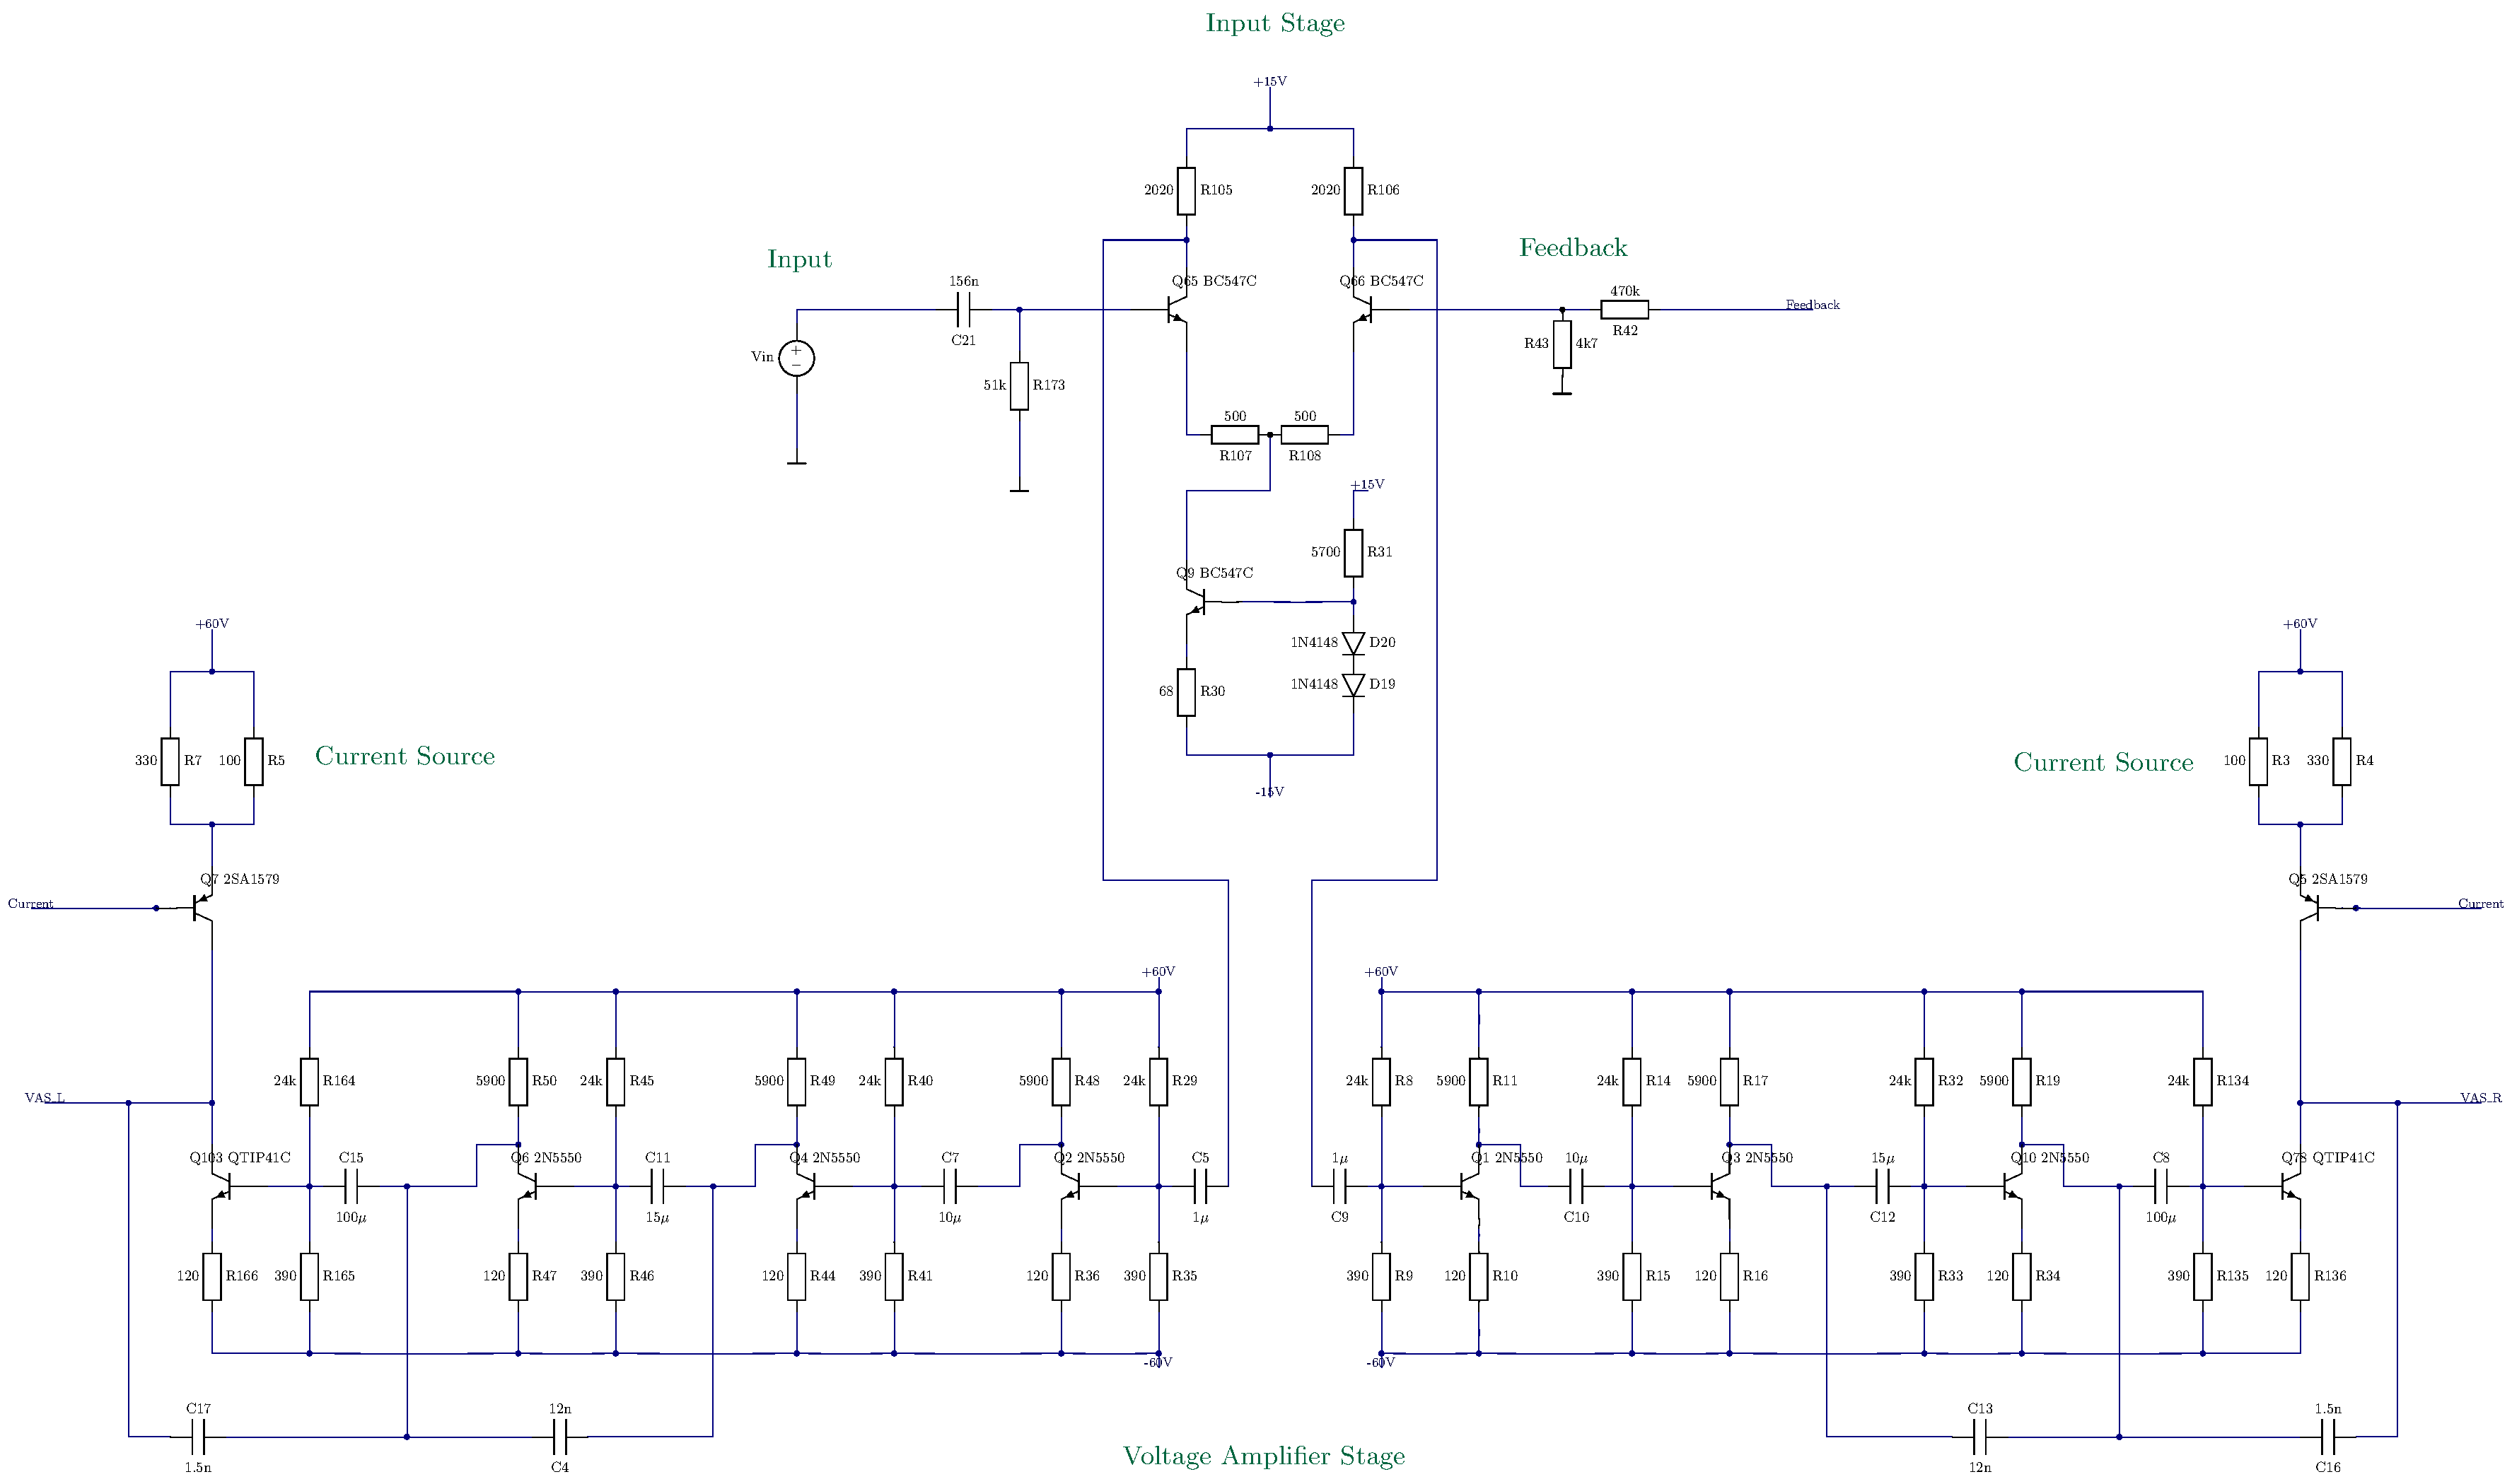
\includegraphics[width=\textwidth]{ImagenesCaracteristicas/TEX1.pdf}
	\caption{Etapas de entrada y amplificación. (Imagen vectorizada la cual no se pixelea)}
	\label{fig:circ}
\end{figure}
 \begin{figure}[H]
\centering
	\includegraphics[width=\textwidth]{ImagenesCaracteristicas/TEX2.pdf}
	\caption{Etapas de salida y carga. (Imagen vectorizada la cual no se pixelea)}
	\label{fig:circ2}
\end{figure}

\begin{itemize}
\item Potencia máxima sin recorte sobre la carga de $1.5k \ W$.
\item Tensión pico sin recorte sobre la carga de $109 \ V$ con una fuente de alimentación de $\pm 60V$.
\item Dos etapas de salida clase AB en configuración puente H.
\item Rendimiento del amplificador del $74.5\%$ posterior al balanceo. (Ver últimos dos items)
\item Respuesta pasabanda en frecuencia para el rango audible con $-3 \ dB$ en $20-20k \ Hz$ respecto a la banda pasante.
\item El circuito se mantiene estable frente a ruido de distinta naturaleza y mantiene una salida sinusoidal.
\item Cuenta con una impedancia de entrada de $50 \ k\Omega$ en toda la banda audible.
\item Implementación con una única fuente partida.
\item Cuenta con una distorsión armónica del $\%$
\item El circuito cuenta con la posibilidad de ajustar el nivel de continua sobre la carga.
\item Permite calibrar el nivel de continua en reposo sobre los transistores de salida.

\end{itemize}



\section{Etapa de Entrada}
	\label{inputstage}
	\documentclass[a4paper]{article}
\usepackage[utf8]{inputenc}
\usepackage[spanish, es-tabla, es-noshorthands]{babel}
\usepackage[table,xcdraw]{xcolor}
\usepackage[a4paper, footnotesep = 1cm, width=20cm, top=2.5cm, height=25cm, textwidth=18cm, textheight=25cm]{geometry}
%\geometry{showframe}

\usepackage{tikz}
\usepackage{amsmath}
\usepackage{amsfonts}
\usepackage{amssymb}
\usepackage{float}
\usepackage{graphicx}
\usepackage{caption}
\usepackage{subcaption}
\usepackage{multicol}
\usepackage{multirow}
\setlength{\doublerulesep}{\arrayrulewidth}
\usepackage{booktabs}

\usepackage{hyperref}
\hypersetup{
    colorlinks=true,
    linkcolor=blue,
    filecolor=magenta,      
    urlcolor=blue,
    citecolor=blue,    
}

\newcommand{\quotes}[1]{``#1''}
\usepackage{array}
\newcolumntype{C}[1]{>{\centering\let\newline\\\arraybackslash\hspace{0pt}}m{#1}}
\usepackage[american]{circuitikz}
\usetikzlibrary{calc}
\usepackage{fancyhdr}
\usepackage{units} 

\graphicspath{{../Calculos-Potencia/}{../Caracteristicas/}{../Consideraciones/}{../Gain-Stage/}{../Input-Stage/}{../Output-Stage/}{../Simulaciones/}{../Alimentacion/}{../Conclusiones/}}

\pagestyle{fancy}
\fancyhf{}
\lhead{22.12 Electrónica II}
\rhead{Mechoulam, Lambertucci, Rodriguez, Londero, Scala}
\rfoot{Página \thepage}

\begin{document}

\subsection{Introducción}

La etapa de entrada de un amplificador cumple con la función de restar a la entrada la señal proveniente de la realimentación, para así obtener la señal deseada de error, a partir de la cual se confecciona la salida del sistema.

\subsection{Distorsión}

La distorsión puede ser provocada o provenir de distintas fuentes. Los amplificadores que se valen del uso de pares diferenciales como entrada se caracterizan por poseer un bajo offset de continua, dado a la cancelación de los voltages de $V_{BE}$. Pero mucho más notorio e importante es que la corriente de mantenimiento no atraviesa la red de realimentación. Finalmente, una ventaja también a destacar es que posee una linealidad superior a las entradas basadas en un solo transistor. Se puede observar la comparación de distorsión entre una etapa diferencial frente a una individual en la Figura (\ref{fig:thd1}).

Es muy importante reflejar que esta etapa debe la que posee la mínima distorsión, por sobre las demás, ya que las señales que maneja son pequeñas, dándose el aumento de estas en la etapa de amplificación.    

%, trim = {0 0 0 20},clip
\begin{figure}[H]
\centering
	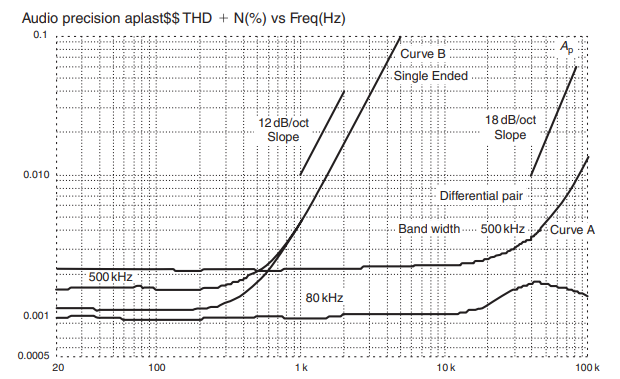
\includegraphics[width=0.6\textwidth]{ImagenesInput-Stage/thd1.PNG}
	\caption{Comparación de THD en función de la frecuencia.}
	\label{fig:thd1}
\end{figure}

Si bien, seleccionando adecuadamente las resistencias del circuito se puede balancear el par, quedan pendientes ciertos parámetros. Las corrientes de colectores deben ser lo más similares posibles. Debe existir una precisión del $1\%$ o mejor para poder optimizar la linealidad del la etapa, y de esta forma, reducir la distorsión en altas frecuencias.
\begin{figure}[H]
\centering
	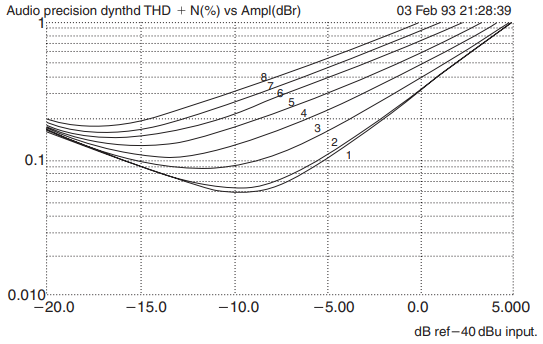
\includegraphics[width=0.6\textwidth]{ImagenesInput-Stage/thd2.PNG}
	\caption{THD en función de la entrada (en $dBu$, nivel de referencia $0.7746 \ V$) al variar el balance de la corriente del colector . Número de curva y distorsión especificadas en la Tabla (\ref{tab:thd2}).}
	\label{fig:thd2}
\end{figure}

\begin{table}[H]
\centering
\begin{tabular}{cc}
\hline
\textbf{Número de curva} & \textbf{Variación $\mathbf{I_C}$ [\%]} \\ \hline
1                        & 0                    \\
2                        & 0.5                  \\
3                        & 2.2                  \\
4                        & 3.6                  \\
5                        & 5.4                  \\
6                        & 6.9                  \\
7                        & 8.5                  \\
8                        & 10             		\\
\hline
\end{tabular}
\caption{Número de curva y distorsión de la Figura (\ref{fig:thd2}).}
\label{tab:thd2}
\end{table}

Una opción valida (e implementada en este diseño) se basa en el uso de una fuente de corriente compensada para polarizar el par. Además, se emplean resistencias en los emisores para ajustar dicho parámetro. Es importante recordar que dichos elementos no deben ser lo suficientemente grandes como para que afecte el ruido térmico\footnote{D. Self, Audio Power Amplifier Design Handbook, 5ta ed. Kidlington: Elsevier Science, 2014.}.  

\subsection{Linealidad y corriente de colector}

La transconductancia aumenta con la corriente de colector. Elevar este último parámetro es posible y relativamente sencillo. Una técnica empleada para poder mejorar la linealidad en altas frecuencias consiste en aumentar la corriente mencionada para luego reducirla a través del lazo de realimentación negativa. Esta no linealidad es atribuida a la resistencia del $R_E$ del emisor, la cual no es una resistencia física, sino que una resultante de la expresión de la pendiente de la corriente de colector. 

La corriente de mantenimiento a la entrada es uno de los parámetros que define el máximo slew rate (SR). Otro factor importante que lo limita es el polo dominante proveniente del capacitor de Miller. Este último es solucionado por los requerimientos que se deben cumplir para conseguir la estabilidad. Por otro lado, aumentar la corriente de colector puede aumentar el factor de SR sin afectar la estabilidad, siempre y cuando, la transconductancia se mantenga en el valor deseado. 

A pesar de ello, existen límites para esta corriente. El aumento de las corrientes de bias, como la caída de tensión a través de las resistencias son algunos ejemplos. El factor más limitante es la potencia disipada a lo largo de esta etapa, ya que no siempre deja margen para incrementar la $I_C$. 

%Se colocó un buffer a ambas salidas del par diferencial. De esta forma se garantiza que las impedancias vistas a la salida de la etapa de entrada son pequeñas y se consigue una mejor adaptación de cargas.

\subsection{Ruido}
El ruido existente en la etapa de entrada surge de los componentes activos y las resistencias que se presentan en la entrada. Las condiciones de operación de los transistores se encuentran limitadas por los factores de SR y linealidad. Por otro lado, ya que el ruido es una función que dependen de $I_C$, bastan con ajustar dicho parámetro para poder reducir el ruido. 

Además de reducir las resistencias existentes en la etapa de entrada para así reducir el ruido térmico existente, es posible realizar el mismo efecto haciendo lo mismo con la resistencia observada a la salida del lazo de realimentación negativa. Este último paso es más delicado ya que puede generar grandes cambios en el sistema. 

%Noise performance is, however, closely bound up with source impedance, and we need to define this before device selection.

\subsection{Limitación en banda}
Se sabe que  existen etapas que acumulan cambios de la fase, siendo estas las altas frecuencias, las cuales tienden a ser más inestables y generar oscilaciones. Es así que se puede llegar a dañar los dispositivos a la salida del sistema por sobrecalentamiento, entre otros motivos. Esto es causado por la distorsión del amplificador y el incremento de la ganancia de lazo abierto. Limitar en banda esta ganancia evita que la señal del realimentador.

\subsection{Calculo de componentes}
Para poder seleccionar los elementos y parámetros que componen la etapa de entrada, se comenzó recorriendo la malla del par. Fijando las caídas de tensión $V_{CE} = 10 \ V$ , se obtiene:
\begin{equation}
	15 \ V - \frac{I_O}{2} R_C - 10 \ V - 10 \ V - 0.7 \ V + 15 \ V = 0
\end{equation}

Ya que see polariza ambos transistores por una fuente de corriente compensada, se obtiene para esa configuración la siguiente ecuación:
\begin{equation}
	-15 \ V - 2V_{D} + V_{BE} + 15 \ V = I_O R 
\end{equation}

Además, se coloca un preset en los emisores del par para poder ajustar la corriente que circula, en caso de ser necesario. Dado esto último, la ganancia del par diferencial con el preset viene dada por la expresión:
\begin{equation}
	\Delta V_D = \frac{h_{fe} R_D}{2 h_{ie} + h_{fe} R_V} = \frac{R_D}{2 \frac{V_T}{I_C} + R_V}
\end{equation}

Sabiendo que la resistencia del colector se encuentra en paralelo con una resistencia de $390 \ \Omega$, y mediante el uso de las ecuaciones previamente mencionadas, se obtienen los siguientes valores de interés:

\begin{table}[H]
\centering
\begin{tabular}{cccc}
\hline
$\mathbf{I_O}$ & $\mathbf{R}$  & $\mathbf{R_C}$ & $\mathbf{R_E}$ \\	\hline
$-9.12 \ mA$   & $68 \ \Omega$ & $2 \ k\Omega$  & $1 \ k\Omega$ \\
\hline
\end{tabular}
\caption{Parametros de la etapa de entrada.}
\end{table}


\end{document}
		
\section{Etapa de Ganancia}
	\label{gainstage}
	

\subsection{Introducción}
La etapa de amplificación de tensión (o VAS) a menudo es considerada como la etapa más crítica de un amplificador de potencia , dado que no solo provee la ganancia de tensión sino que también debe manejar todo el rango de la tensión de salida. Esto indicaría que puede jugar un rol significativo en la distorsión armónica de la señal, sin embargo un VAS bien diseñado contribuye relativamente poco a la distorsión total, e incluso si se tomasen pasos extra para intentar linealizar aún más la salida, estas contribuciones comparadas con las hechas en una etapa de entrada, son completamente despreciables.\\

El primer diseño que se pensó fue un emisor común que se observa a continuación que si bien  cuenta con varios problemas estos van  a ser sorteados en las siguientes lineas.
\begin{figure}[H]
\centering
	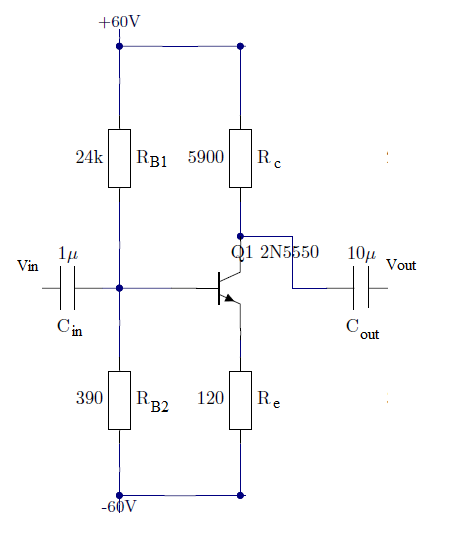
\includegraphics[width=0.7\textwidth]{ImagenesGain-Stage/ec1.png}
	\caption{Primer diseño Emisor Común}
	\label{fig:ec1}
\end{figure}

El primer problema que se afrontó fue el de limitar la ganancia de altas frecuencias.
Para esto se introduce una linea de realimentación negativa utilizando $C_{dom}$ el cual limita la ganancia de altas frecuencia y así asegura mayor estabilidad.
 \begin{figure}[H]
\centering
	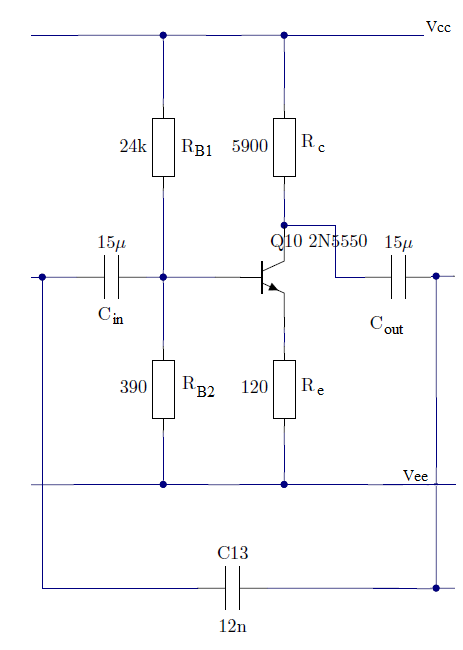
\includegraphics[width=0.7\textwidth]{ImagenesGain-Stage/ec2.png}
	\caption{Segundo diseño Emisor Común}
	\label{fig:ec2}
\end{figure}
En cuanto al cálculo de $C_{in}$ o $C_{out}$ se buscó que la impedancia para frecuencias medias sea despreciable frente a la impedancia vista desde el colector o la base.\\
Para el caso de $C_{Dom}$ se eligió un valor tal que las altas frecuencias vean un camino de baja impedancia comparado con la entrada del emisor común. De esta manera, las frecuencias altas no serán amplificadas.\\
Es importante que la ganancia a lazo abierto del VAS sea alta, así este puede ser linealizado. Si se intenta aumentar la ganancia del emisor común, se sabe que la ganancia de este está descripto por la ecuación:
\begin{align}
A_{vs}=\frac{-R_D}{R_E}
\end{align}
Por lo que si se quiere subir la ganancia puede subirse el valor de $R_C$, pero esto dado una $I_c$ determinada por la  malla de entrada, provocará que caiga más tensión sobre la resistencia $R_C$ y así consuma un valor de potencia mucho más elevado. Una manera de asegurar una gran ganancia es utilizar una carga activa con una fuente de corriente, así suministrando la corriente necesaria, y mostrando una alta impedancia. \\
Además, se optó por utilizar un acople por fuente de corriente en vez de uno capacitivo con la idea de no introducir singularidades no deseadas en el circuito.
 \begin{figure}[H]
\centering
	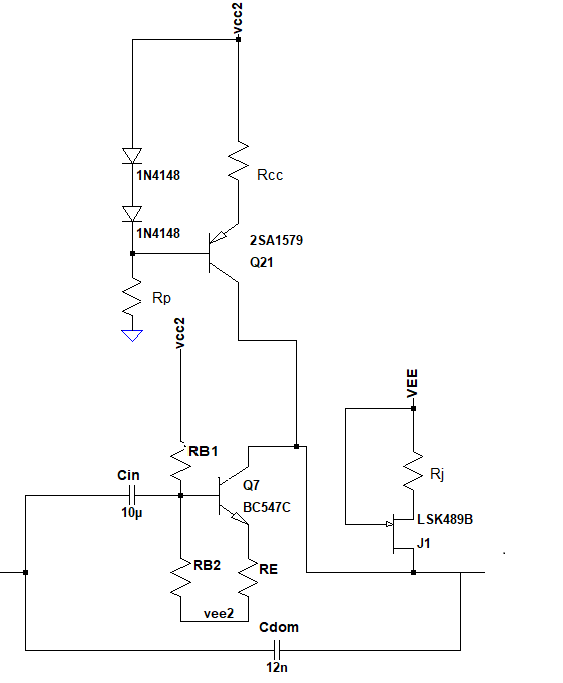
\includegraphics[width=0.7\textwidth]{ImagenesGain-Stage/ec3.png}
	\caption{Tercer diseño Emisor Común}
	\label{fig:ec3}
\end{figure}

Para la fuente de corriente de la carga activa se optó por utilizar una fuente compensada. Mientras que para el acomple se utilizó una fuente implementada con JFET, debido a que en esa zona el circuito tiene la máxima variación de tensión, lo cual si se hubiese implementado con una fuente con BJT podría tener problemas de Saturación / Corte.\\
El transistor se le impuso una tensión de VCE de $\frac{V_{cc}+V_{ee}}{2}$ al igual que un valor de corriente Ic = 10mA, al igual que optar por una resistencia de emisor baja.\\
Los valores utilizados para el circuito responden a las siguientes ecuaciones:
\begin{align}
R_{B2}= \frac{V{Re}+V_{be}}{I_{RB}} \approx 390 \Omega |_{IRb=5mA \  \ \wedge \ \  Vre=1.2V}
\end{align}
\begin{align}
R_E=\frac{I_{Rb}\cdot R_{B2}-2V_{be}}{I_c}=120\Omega
\end{align}
\begin{align}
R_{B1}= \frac{V_{cc}+V_{ee}-I_{Rb}\cdot R_{B2}) }{I_{Rb}=24k\Omega}
\end{align}
Luego para la fuente compensada se obtuvo un valor para la resistencia $R_{cc}$, tal que suministre los $10 \ mA$ al colector del transistor.

\begin{align}
R_{cc}=\frac{V_{be}}{I_c}\approx 76\Omega
\end{align}
También se obtiene el parámetro de la impedancia de salida de la fuente compensada la cual es de aproximadamente:
\begin{align}
R_{of} = (R_cc // hie^*)+(1+hfe^* )\cdot rce
\end{align}
En cuanto a la compensación por corriente se optó por el transistor UJ3N065080K3S debido a que puede manejar el rango de tensiones de la salida y puede proveer una corriente suficiente, si bien este era el transistor ideal, el subcircuito encontrado en linea parece no funcionar correctamente por lo que se utilizo el LSK489B para la simulación, pero ese transistor sería el utilizado en la realidad. En cuanto a la  elección de la resistencia del Jfet, se consideraron los parametros $V_p \ , \ I_{dss}$.
\begin{align}
I_D=-\frac{V_{GS}}{R_j}
\end{align}
El valor de la corriente de drain que se necesitará será la corriente la cual se fugaría del VAS hacia la etapa de salida al no estar presente el capacitor, la cual es de un valor de $\approx 5 \ mA$.
\begin{align}
I_D= I_{DSS} \cdot \left(1-\frac{V_{GS}}{V_P} \right)^2
\end{align}

De aquí se obtiene $R_j \approx 65 \ \Omega$.\\
La fuente de corriente de acople posee además una segunda característica. Esta permite no solo regular el nivel de continua de reposo a la salida de cada clase AB, sino también el nivel de continua de reposo sobre la carga. Basta que ambas salidas en reposo sean iguales para que la continua de reposo sobre la carga sea nula, sin embargo, si no se compensa correctamente con esta fuente el nivel de continua en reposo a la salida de cada clase AB, se consumirá una gran potencia lo que disminuirá considerablemente el rendimiento del amplificador, por más que los parlantes no se dañen debido a la simetría del circuito.

Como última consideración se optó por poner 3 etapas amplificadoras como la de la Figura (\ref{fig:ec1}) previo al diseño de la Figura (\ref{fig:ec3}) con la intención de aumentar la ganancia del bloque A tal  que valga que $\alpha \cdot \beta \gg 1$ dado que $\beta$ será de un valor muy pequeño para lograr llegar a disipar como máximo $1 \ kW$ sobre la carga.


%\begin{align}
%\end{align}

	
\section{Etapa de Salida}
	\label{outputstage}
	\documentclass[a4paper]{article}
\usepackage[utf8]{inputenc}
\usepackage[spanish, es-tabla, es-noshorthands]{babel}
\usepackage[table,xcdraw]{xcolor}
\usepackage[a4paper, footnotesep = 1cm, width=20cm, top=2.5cm, height=25cm, textwidth=18cm, textheight=25cm]{geometry}
%\geometry{showframe}

\usepackage{tikz}
\usepackage{amsmath}
\usepackage{amsfonts}
\usepackage{amssymb}
\usepackage{float}
\usepackage{graphicx}
\usepackage{caption}
\usepackage{subcaption}
\usepackage{multicol}
\usepackage{multirow}
\setlength{\doublerulesep}{\arrayrulewidth}
\usepackage{booktabs}

\usepackage{hyperref}
\hypersetup{
    colorlinks=true,
    linkcolor=blue,
    filecolor=magenta,      
    urlcolor=blue,
    citecolor=blue,    
}

\newcommand{\quotes}[1]{``#1''}
\usepackage{array}
\newcolumntype{C}[1]{>{\centering\let\newline\\\arraybackslash\hspace{0pt}}m{#1}}
\usepackage[american]{circuitikz}
\usetikzlibrary{calc}
\usepackage{fancyhdr}
\usepackage{units} 

\graphicspath{{../Calculos-Potencia/}{../Caracteristicas/}{../Consideraciones/}{../Gain-Stage/}{../Input-Stage/}{../Output-Stage/}{../Simulaciones/}{../Alimentacion/}{../Conclusiones/}}

\pagestyle{fancy}
\fancyhf{}
\lhead{22.12 Electrónica II}
\rhead{Mechoulam, Lambertucci, Rodriguez, Londero, Scala}
\rfoot{Página \thepage}

\begin{document}

\subsection{Introducción}

La etapa de salida de un amplificador de audio se encarga de entregar la corriente necesaria a la carga para conseguir la característica de potencia buscada en el amplificador; sin así distorsionar demasiado a la señal, para preservar el THD para el cual se trabajó tanto para disminuir en las etapas anteriores.

Por un lado, se puede utilizar tecnología FET, sin embargo, estos presentan muy pocas ventajas frente a desventajas con otras tecnologías. Una alternativa aún utilizada son las válvulas, que quedan descartadas al no ser relevante en este trabajo. Otra alternativa, mucho más popular, es usar tecnología BJT, la cual será nuestra opción. 

Existen varias clases de etapa de salidas distintas, entre ellas A, con una alta linealidad pero muy baja eficiencia; clase B, la cual soluciona el problema de la eficiencia, al costo de la distorsión por crossover; la clase AB, un compromiso entre ambas; variaciones de la popular clase AB, como la clase G que utiliza 4 rieles de alimentación distintos, y muchas más.
En el amplificador de audio diseñado se utilizará clase AB al ser una consideración de diseño.

Dentro de la clase AB existen muchas topologías distintas, cada una con sus respectivas ventajas y desventajas. Una de ellas es la topología EF (\textit{emitter-follower}) compuesta por un seguidor por emisor o dos en cascada. En esta última, un transistor funciona como \textit{driver}, generalmente situado en un punto Q muy estable. Este transistor proporciona la corriente de base al siguiente, generalmente un transistor de potencia, por el cual fluye la corriente que se le entrega a la carga. Dentro de esta topología existen tres tipos mostrados en la Figura (\ref{fig:ef}). En el tipo 1 los resistores de emisor se conectan a la salida. Estos resistores colocan al driver en un punto Q estable. El tipo 2 posee la ventaja de ahorrarse un resistor, colocando uno solo entre los emisores de los transistores. Además, los transistores nunca se polarizarán en inversa al pasar de un semiciclo al otro. En el tipo 3, se conectan los resistores a los rieles de alimentación, lo cual puede mejorar el apagado de altas frecuencias.

%, trim = {0 0 0 20},clip
\begin{figure}[H]
\centering
	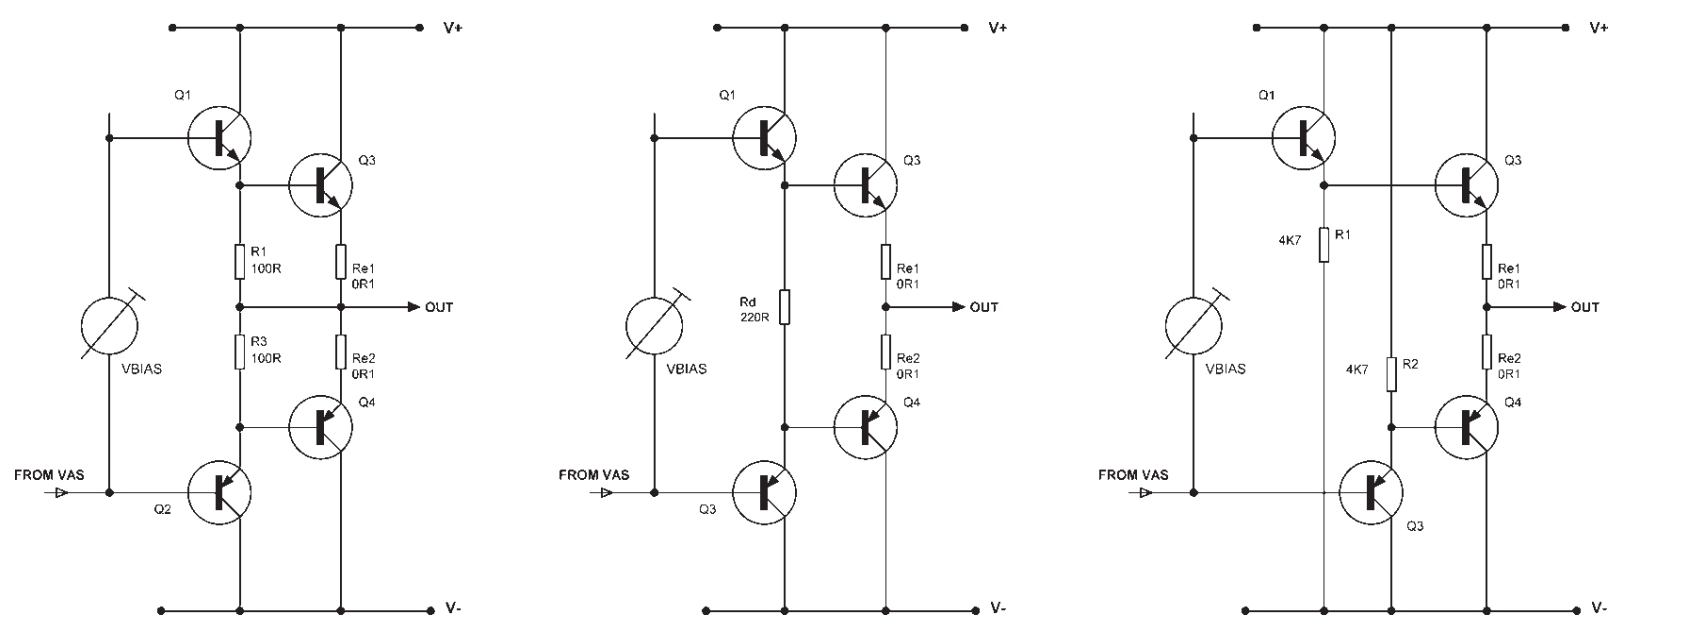
\includegraphics[width=\textwidth]{ImagenesOutput-Stage/pag143-EF.png}
	\caption{Tipos de configuraciones emitter follower. D. Self, Audio Power Amplifier Design Handbook, 5th, p. 143.}
	\label{fig:ef}
\end{figure}


Otra configuración involucra los pares Sziklai, Quasi-Darlington o también llamados par de realimentación, dado que ahora el driver se coloca de manera tal que este compare la tensión a la salida con la entrada, lo cual aumenta la linealidad. Además, como el Vbe del transistor de salida se encuentra dentro del lazo de realimentación, se observa una estabilidad térmica mayor.

%, trim = {0 0 0 20},clip
\begin{figure}[H]
\centering
	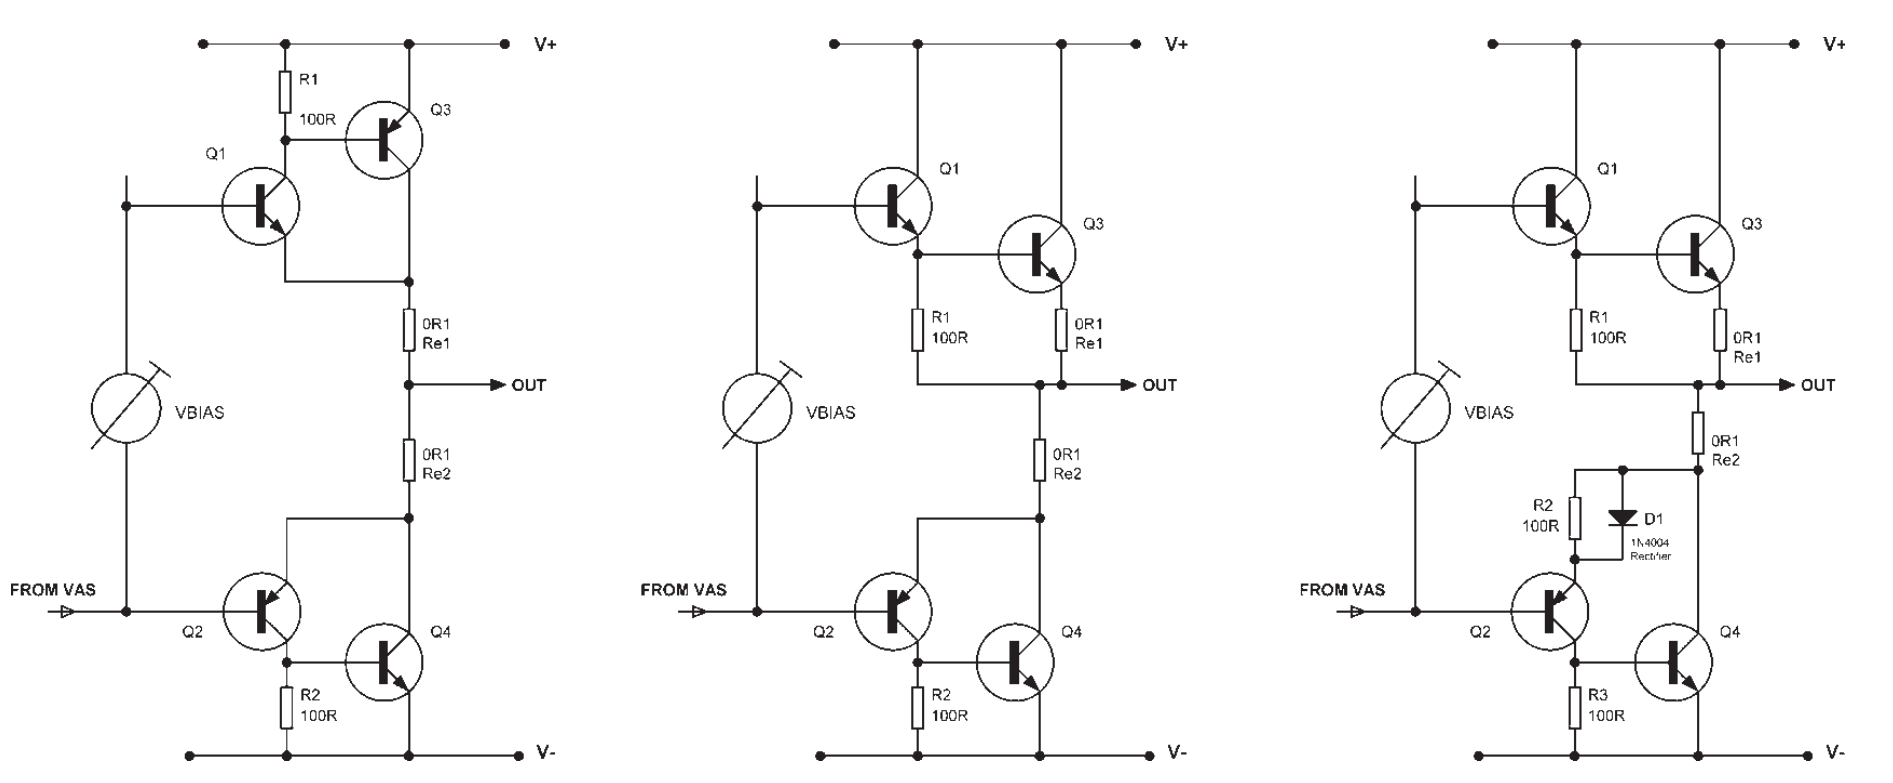
\includegraphics[width=\textwidth]{ImagenesOutput-Stage/pag145-CFP.png}
	\caption{Tipos de configuraciones de par de realimentación. D. Self, Audio Power Amplifier Design Handbook, 5th, p. 145.}
	\label{fig:cfp}
\end{figure}

Una topología la cual en el pasado era casi obligatoria por la falta de transistores PNP de potencia complementarios a los NPN, es la casi complementaria. En esta configuración solamente se reemplaza por un par Quasi-Darlington a los transistores PNP. Esta topología presenta una linealidad mucho menor y no será utilizada, aunque existen varios arreglos a la simetría, como por ejemplo utilizando un diodo de Baxandall.

Naturalmente surge al analizar estas etapas de salida la idea de colocar tres transistores en cascada, o más. De ahí surge la topología basada en triples, como la Triple EF. Esta configuración presenta mayor linealidad a alta potencias, un punto Q más estable para los transistores \textit{pre-drivers}, los que proporcionan la corriente a los drivers, debido a que estos manejarán una corriente menor y disiparán menor potencia. Además, al poseer una ganancia de corriente mayor, la etapa de ganancia de tensión deberá proporcionar corrientes menores. En la Figura (\ref{fig:triples}) se observan distintas configuraciones triples posibles.

%, trim = {0 0 0 20},clip
\begin{figure}[H]
\centering
	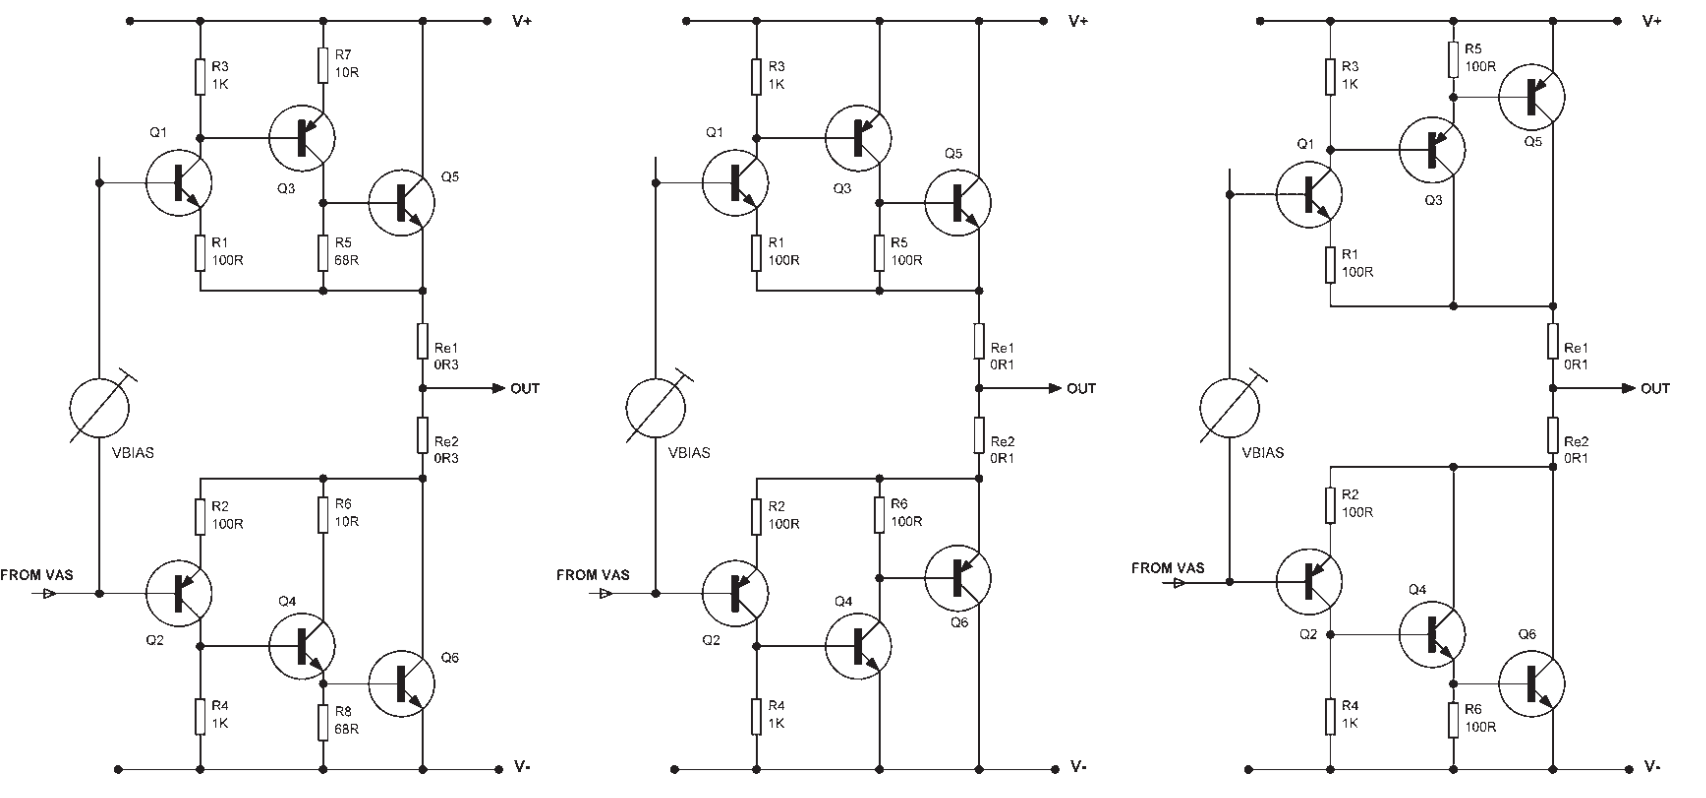
\includegraphics[width=\textwidth]{ImagenesOutput-Stage/pag145-triples.png}
	\caption{Algunos tipos de configuraciones basadas en triples. D. Self, Audio Power Amplifier Design Handbook, 5th, p. 145.}
	\label{fig:triples}
\end{figure}

\subsubsection{Topología Utilizada}
Debido a la alta potencia que se deberá disipar sobre la carga, que al ser de tan solo $8 \ \Omega$ provoca corrientes muy grandes, se decidió utilizar una topología basadas en triples detallado en la Figura (\ref{fig:triples}). Esto permite, como ya descrito antes, utilizar transistores de media potencia como pre-drivers que tanto permanezcan a una temperatura estable como posean una pequeña excursión en corriente, lo que aumenta la linealidad de la etapa de salida. Luego, el transistor driver y de salida serán de potencia. Se utilizará una configuración con pares de realimentación para aumentar aún más la linealidad.

 %, trim = {0 0 0 20},clip
\begin{figure}[H]
\centering
	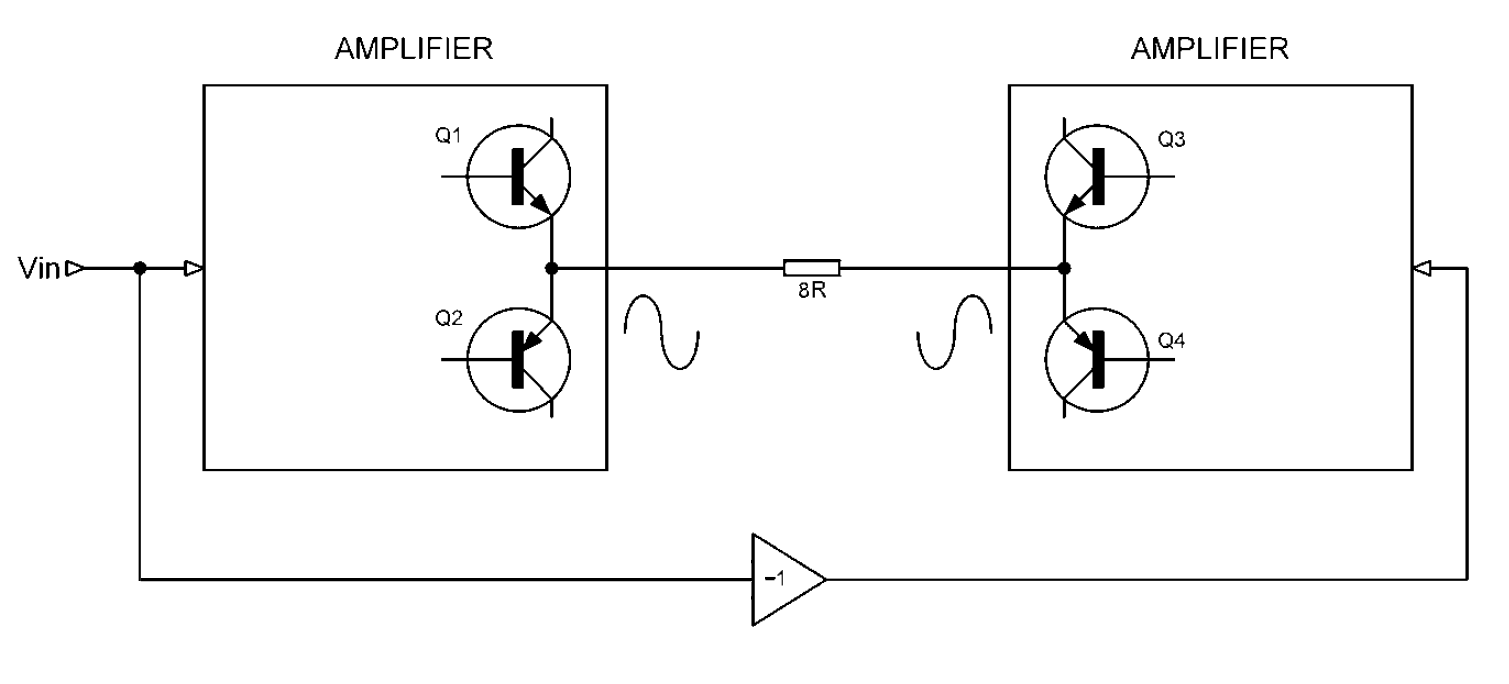
\includegraphics[width=0.7\textwidth]{ImagenesOutput-Stage/pag38-bridge_2.png}
	\caption{Puenteo de la carga con las etapas de salida. D. Self, Audio Power Amplifier Design Handbook, 5th, p. 38.}
	\label{fig:bridge}
\end{figure}

Por otro lado, se utilizaron dos etapas de salida idénticas pero en contra-fase con la carga entre la salida de ambas. Esto permite (debido a que el amplificador diseñado será para una carga mono y no estéreo) duplicar la tensión sobre la carga y así cuadriplicar la potencia disipada sobre esta.
Como la potencia disipada será muy alta, se decidió utilizar además una técnica muy frecuentemente empleada en amplificadores de audio comerciales, la cual consiste en colocar varios transistores de salida en paralelo, encontrando en amplificadores profesionales hasta incluso doce de ellos o más. El cálculo del número de pares de transistores en paralelo se detallará en la sección de potencia y serán de 6 pares por lado.

 %, trim = {0 0 0 20},clip
\begin{figure}[H]
 \hspace{-1cm}
	\includegraphics[width=1.1\textwidth]{TEX2.pdf}
	\caption{Circuito diseñado para la etapa de salida. (Imagen vectorizada)}
	\label{fig:output}
\end{figure}

Las resistencias de emisor de los transistores se seleccionaron de acuerdo al libro Audio Power Amplfier Design Handbook de Douglas Self con un valor de $390 \ \Omega$ para los transistores pre-driver, $180 \ \Omega$ para los transistores driver y $0.1 \ \Omega$ para los transistores de salida.  Luego, se utilizaron los transistores $MJ21194$ y $MJ21193$ debido a su uso en amplificadores de audio comerciales de alta potencia y los transistores $2N5550$ y $2N5401$ para los pre-drivers, que, si bien disipan mucho menos que los demas transistores, poseen una gran caída de tensión $V_{CE}$.


\subsubsection{Generador de Bias}

Para el generador de bias se utilizó inicialmente un multiplicador de Vbe compuesto por dos resistencias y un transistor. Sin embargo, resultados experimentales demostraron que este generador de bias fallaba en mantener una tensión constante de bias frente a las grandes variaciones de corriente que egresaban de la etapa de salida. Debido a esto, se utilizó un par de realimentación compensado en vez del transistor, lo cual aumenta el beta total, logrando generar una tensión de bias con una fluctuación alrededor de diez veces menor.

 %, trim = {0 0 0 20},clip
\begin{figure}[H]
\centering
	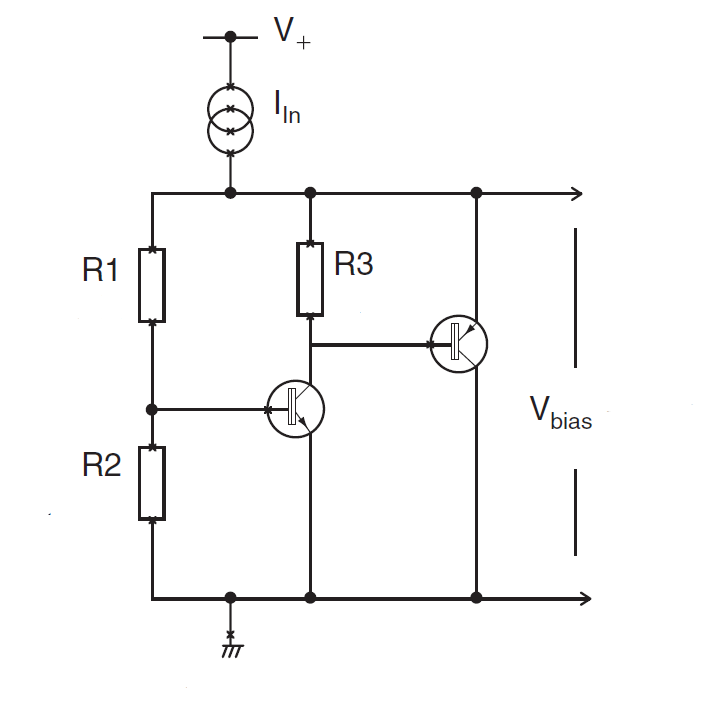
\includegraphics[width=0.4\textwidth]{ImagenesOutput-Stage/pag417-bias.png}
	\caption{Generador de bias utilizado. D. Self, Audio Power Amplifier Design Handbook, 5th, p. 417.}
	\label{fig:bias}
\end{figure}

La corriente que fluye por las resistencias $R_1$ y $R_2$ está gobernada por tanto la caída de $V_{be}$ como por el valor de $R_2$. Imponiendo una corriente de $2 \ mA$ para estas resistencias, se tiene que

\begin{equation}
I_R = \frac{0.6 \ V}{2 \ mA} = 300 \ \Omega
\end{equation}

Luego, dado que se encuentran seis caídas de $V_{be}$, lo cual equivale a $4.2 \ V$, se decidió para poder ajustar el nivel de corriente de reposo de los transistores de salida, tomar ese valor como central y con un trimmer brindar una excursión bilateral frente este valor central. Si el trimmer se coloca en la posición de menor resistencia, habrá una gran distorsión de crossover, mientras que si se coloca en la posición de mayor resistencia habrá una gran corriente de reposo. Teniendo esto en cuenta, y las recomendaciones del libro de Douglas Self, de utilizar un $V_{bias}$ de $3.9 \ V$ para la configuración Triple EF, se tiene que $R_2 = R_{2-fija} + R_{2-trimmer}$. $R_{2-fija} = 1.5 \ k\Omega$ y $R_{2-trimmer} = 500 \ \Omega$ nominales. Esto hará que

\begin{equation}
3.6 \ V < V_{bias} = V_{be}\cdot \frac{R_a + R_b}{R_b} < 4.6 \ V
\end{equation} 

\subsubsection{Fuente de corriente}

Finalmente, se utilizó una fuente de corriente compensada simple en vez de una resistencia para no limitar por corriente a la máxima potencia sin recorte a la salida. Esta fuente de corriente será la que provea de corriente a tanto el generador de Bias como a los transistores pre-driver de salida. Para el valor de la fuente de corriente se decidió utilizar $7 \ mA$ dado que eso brinda suficiente margen entre la corriente de base del transistor pre-driver ($\approx 1 \ mA$) y el generador de bias. Se cedieron alrededor de $6 \ mA$ al generador de bias para no solo dejar una buena corriente de colector en los transistores, sino también dejar una corriente sobre las resistencias para que valga la aproximación de divisor resistivo. Se obtuvo entonces que la resistencia que fija la corriente de la compensada es
\begin{equation}
R_{curr} = \frac{0.7 \ V}{7 \ mA} = 100 \ \Omega
\end{equation}
Finalmente para polarizar correctamente los diodos, como se colocaron cuatro transistores en paralelo a estos, se impuso una corriente mayor a la habitual, de $20 \ mA$. Obteniendo así
\begin{equation}
R_{diod} = \frac{0.7 \ V}{20 \ mA} = 3k3 \ \Omega
\end{equation}

\subsubsection{Resistor sumidero de corriente}

Por esta resistencia fluirá la resta de corrientes entre la proporcionada por la fuente de corriente compensada descrita anteriormente y la fuente de corriente JFET, la cual cumple la función de acople entre el VAS y la etapa de salida, y de ajuste de continua en la carga. Se tiene luego que $7 \ mA - 5 \ mA = 2 \ mA$. Luego,

\begin{equation}
R = \frac{V_{output_{max}}}{I_R} = \frac{45 \ V}{2 \ mA} = 22.5 \ k\Omega 
\end{equation} 

Sin embargo, se comprobó empíricamente mediante simulaciones que un valor de $R = 25 \ k\Omega$ decrece la distorsión armónica sin comprometer mucho el funcionamiento.

\end{document}
	
\section{Alimentación}
	\label{alimentacion}
	
\subsection{Alimentación}
Se eligió utilizar una fuente partida de $\pm60 \ V$  debido a que se buscaba una tensión de salida elevada para obtener un valor de potencia sobre la carga de $\approx 1.5 \ kW$. Para esto, la tensión pico de cada lado del amplificador debe ser de $\approx 53 \ V$. Utilizando $60 \ V$ se llega a un buen compromiso entre tener un margen considerable hasta el recorte para reducir el THD, y el rendimiento del amplificador.\\ 
También se optó por utilizar un segundo riel de alimentación para el par diferencial, teniendo como objetivo optimizar el rendimiento, dado que este trabaja con pequeña señal. Se utilizó un valor de $\pm$ 15V, empleando una resistencia y un diodo zener para proveer esa tensión a partir de la fuente partida principal.
\begin{figure}[H]
\centeringfccc
	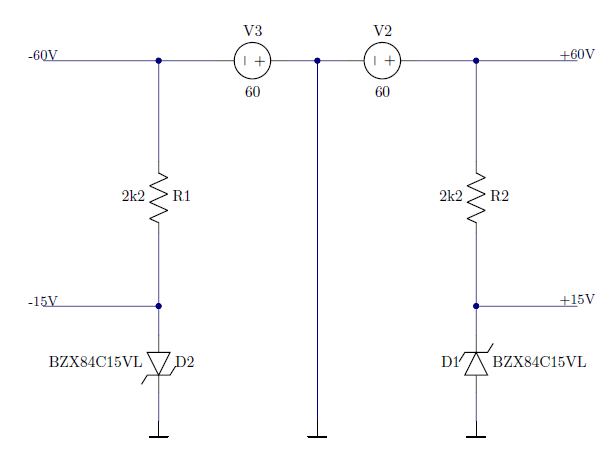
\includegraphics[width=0.7\textwidth]{ImagenesAlimentacion/al.png}
	\caption{Fuente de alimentación}
	\label{fig:alimentacion}
\end{figure}
El diodo seleccionado es uno cuya tensión de zener es de $15 \ V$.
Para el cálculo de la resistencia del diodo se tuvo en cuenta que el diodo quede polarizado con una corriente de mantenimiento de $6 \ mA$ al igual que haya suficiente corriente para que el par diferencial utilice. Teniendo en cuenta la corriente de polarización del par diferencial se llega a la conclusión de que la corriente por la resistencia debe ser de $20 \ mA$.
\begin{align}
R1=\frac{60-V_z}{20mA}= 2k2\Omega
\end{align}


\section{Cálculos de Potencia}
	\label{calculospotencia}
	%\documentclass[a4paper]{article}
\usepackage[utf8]{inputenc}
\usepackage[spanish, es-tabla, es-noshorthands]{babel}
\usepackage[table,xcdraw]{xcolor}
\usepackage[a4paper, footnotesep = 1cm, width=20cm, top=2.5cm, height=25cm, textwidth=18cm, textheight=25cm]{geometry}
%\geometry{showframe}

\usepackage{tikz}
\usepackage{amsmath}
\usepackage{amsfonts}
\usepackage{amssymb}
\usepackage{float}
\usepackage{graphicx}
\usepackage{caption}
\usepackage{subcaption}
\usepackage{multicol}
\usepackage{multirow}
\setlength{\doublerulesep}{\arrayrulewidth}
\usepackage{booktabs}

\usepackage{hyperref}
\hypersetup{
    colorlinks=true,
    linkcolor=blue,
    filecolor=magenta,      
    urlcolor=blue,
    citecolor=blue,    
}

\newcommand{\quotes}[1]{``#1''}
\usepackage{array}
\newcolumntype{C}[1]{>{\centering\let\newline\\\arraybackslash\hspace{0pt}}m{#1}}
\usepackage[american]{circuitikz}
\usetikzlibrary{calc}
\usepackage{fancyhdr}
\usepackage{units} 

\graphicspath{{../Calculos-Potencia/}{../Caracteristicas/}{../Consideraciones/}{../Gain-Stage/}{../Input-Stage/}{../Output-Stage/}{../Simulaciones/}{../Alimentacion/}{../Conclusiones/}}

\pagestyle{fancy}
\fancyhf{}
\lhead{22.12 Electrónica II}
\rhead{Mechoulam, Lambertucci, Rodriguez, Londero, Scala}
\rfoot{Página \thepage}
%%
%\begin{document}

%\subsection{Introducción}

\subsection{Simulación de  rendimiento}
El rendimiento esta definido como:
\begin{align}
\eta = \frac{P_{RL}}{P_{vcc}+P_{vee}}
\end{align}
Teniendo en cuenta que la potencia para las señales senoidales se toma la potencia eficaz, siendo esta:
\begin{align}
P_{R}=V_{R-RMS}\cdot I_{R-RMS} =\frac{\hat{V_{R}}}{\sqrt{2}} \cdot \frac{\hat{I_{R}}}{\sqrt{2}}
\end{align}
Finalmente fue simulado el rendimiento obteniendo los siguientes valores:
\begin{align}
\eta=\frac{1083 / 2 W}{ 2\cdot 18 W + 2 \cdot 690 /2}\approx 74.5 \%
\end{align}

\subsection{Etapa de ganancia}
Para el cálculo de la potencia de este bastará con realizar el cálculo\footnote{Los valores de corriente $I_c$ y tensión $V_{ce}$ son los calculados en la etapa de ganancia}:
\begin{align}
P_{ec4}\approx\left[V_{ce-cc} + \frac{\hat{V_{ce-ac}}}{\sqrt{2}}\right]\cdot I_c\approx 540 \ mW
\end{align}
Dado a la potencia media que disipa y la tensión que debe manejar se eligió un TIP41C, el cual puede manejar este trabajo sin disipador.
En cuanto a las otras tensiones $V_{ce}$ de los transistores debido a que no trabajan con señales tan grande se aproxima la potencia disipada a la de continua.
\begin{align}
P_{ec-123}\approx V_{ce-cc} \cdot I_c \approx 597 \ mW
\end{align}
Este transistor todavía se encuentra dentro de la potencia que puede disipar sin disipador.
Por otro lado, para las resistencias de colector de los emisores comunes será una potencia de:
\begin{align}
P_{Rc}= I_c^2 \cdot R_c \approx 0.55 \ W
\end{align}

Para la carga a activa bastará con realizar el producto de la tension de juntura por la corriente.
\begin{align}
P_{CS}\approx\left[V_{ce-cc} + \frac{\hat{V_{ce-ac}}}{\sqrt{2}}\right]\cdot I_c\approx  632\ mW
\end{align}
En cuanto a este transistor cabe destacar que tampoco es necesario el uso de un disipador.
\subsection{Etapa de entrada}
Se calcula la potencia disipada por la etapa de entrada. Para los transistores del par diferencial, sabiendo $I_C$ y $V_{CE}$ (y despreciando la corriente de base) se obtiene aproximadamente: 
\begin{equation} 
	P_{Q65} = P_{Q66} \approx V_{CE} I_C \approx 30 \ mW
\end{equation}
para cada uno, mientras que para el transistor de la fuente de corriente
\begin{equation} 
	P_{Q9} \approx V_{CE} I_C \approx 106.23 \ mW
\end{equation}

Para el conjunto de las resistencias $R_V$ ($R_{107} + R_108$), $R_{105}$ y $R_{106}$, se obtiene una potencia de
\begin{equation} 
	P_{R105} + P_{R106} + P_{RV} \approx  I_C^2 \left(R_{105} + R_{106} + R_V \right) \approx 111.57 \ mW
\end{equation}

Para la resistencia $R_{30}$, se calculó 
\begin{equation} 
	P_{R30} \approx  I_O^2 R_{30} \approx 6.02 \ mW
\end{equation}
mientras que para $R_{31}$
\begin{equation} 
	P_{R31} \approx  \frac{\left( 30 \ V - 1.7 \ V \right)^2}{R_{31}} \approx 143.50 \ mW
\end{equation}

Luego, para los diodos $D_{19}$ y $D_{20}$, conjuntamente se calcula una potencia de
\begin{equation} 
	P_{D1} + P_{D2} \approx  \left( 1.7 \ V \right) \frac{30 \ V - 1.7 \ V}{R_{31}} \approx 7.02 \ mW
\end{equation}
 
Finalmente, sumando todas las potencias disipadas, se obtiene total de $404.34 \ mW$.  
%Este valor se contrasta contra los $433.08 \ mW$ obtenidos de la simulación. Es entendible la diferencias

%\end{document}
	
	
\section{Simulaciones}
	\label{simulaciones}
	
\subsection{Introducción}
Se realizaron simulaciones en LTSpice del circuito propuesto, así también se comprobó que los resultados teóricos concuerdan con las simulaciones, ademas se tuvo especial cuidado a la hora de evaluar que transistores y resistores usar en las etapas tal que no haya problemas de potencia, aqui se muestran las tensiones y potenicas relevantes del circuito en cuanto a la elección crítica de componentes.\\
Comenzando por los emisores comunes la potencia se encuentra cerca del máximo y la tensión Vce en un rango seguro.

\begin{figure}[H]
	\centering
	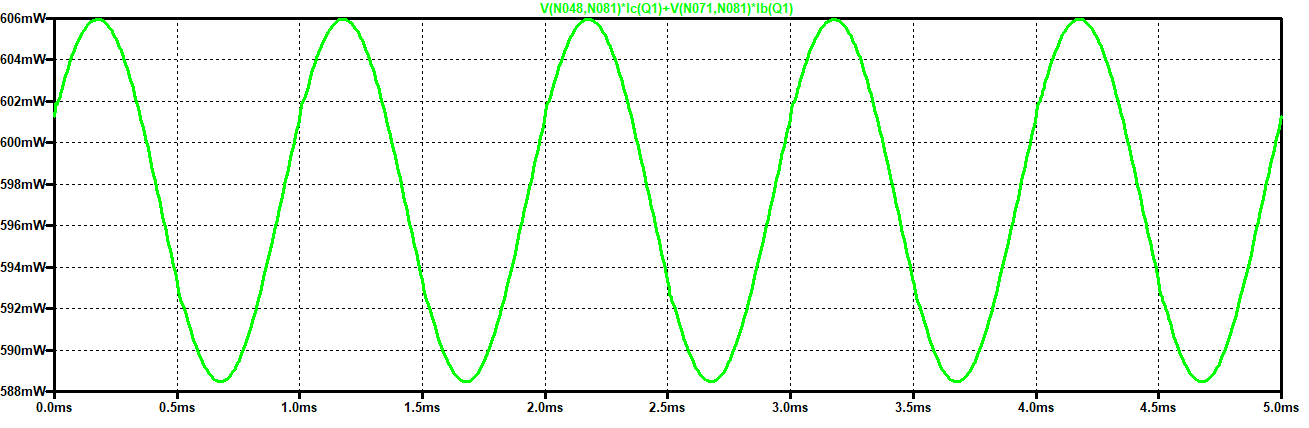
\includegraphics[width=0.8\textwidth]{ImagenesSimulaciones/PEC1.png}
		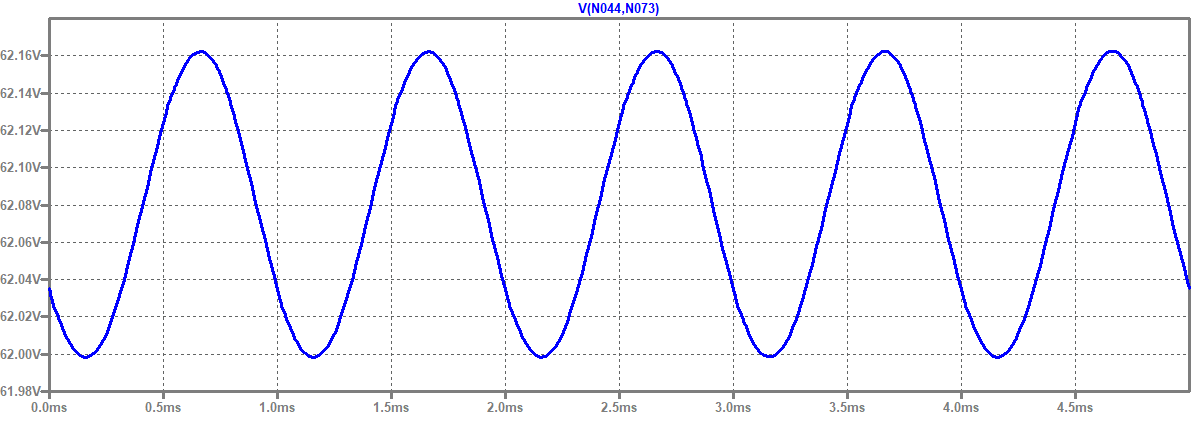
\includegraphics[width=0.8\textwidth]{ImagenesSimulaciones/VEC1.png}
	\caption{Potencia y tensión sobre un emisor común sin carga activa.}
	\label{fig:pec1}
\end{figure}También se cuenta con que la potencia disipada por las resistencias de colector son cercanas al medio watt, por lo que las resistencias a utilizar son de medio watt.\\
Luego el úlitmo emisor común, el cual tiene la mayor ganancia de todos, es razonable esperar que disipe mas potencia y en efecto así es, por eso la necesidad de utilizar un transistor de mayor potencia para este ademas de que este manejara la máxima variación de tensión.

\begin{figure}[H]
	\centering
	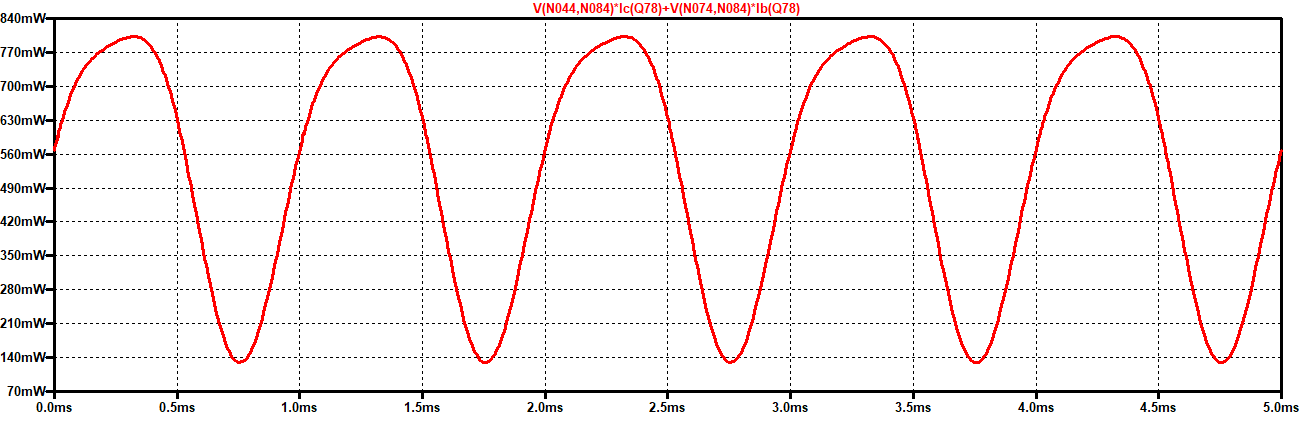
\includegraphics[width=0.8\textwidth]{ImagenesSimulaciones/PECF.png}
		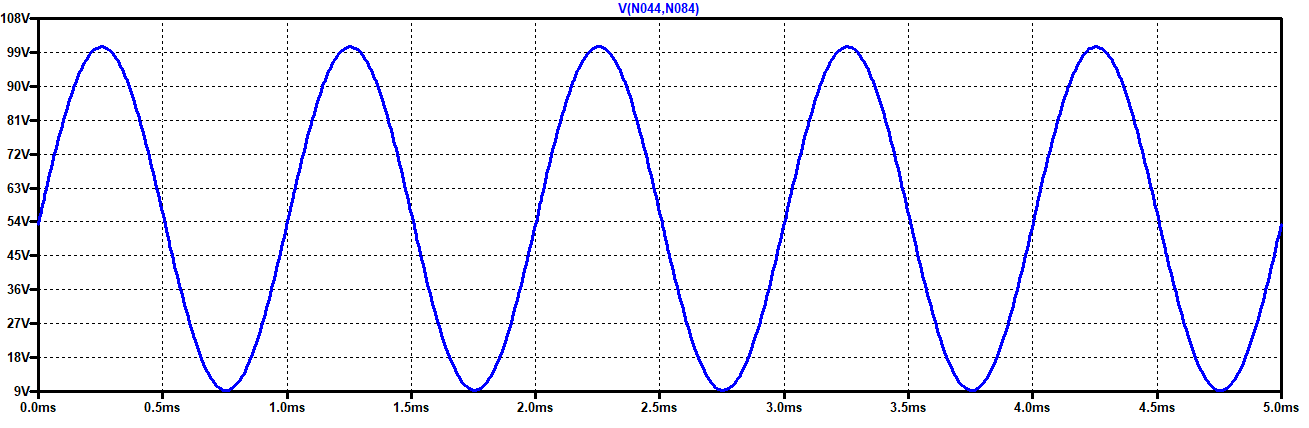
\includegraphics[width=0.8\textwidth]{ImagenesSimulaciones/VECF.png}
	\caption{Potencia y tensión sobre un emisor común con carga activa.}
	\label{fig:pecf}
\end{figure}
%% potencai fuente de corriente de la carga activa
En cuanto a la carga activa, dado que se encuentra en el colector del transistor va a  sufrir también una gran variación de tensión por lo que se necesita un transistor que pueda manejar dicha tensión.
\begin{figure}[H]
	\centering
	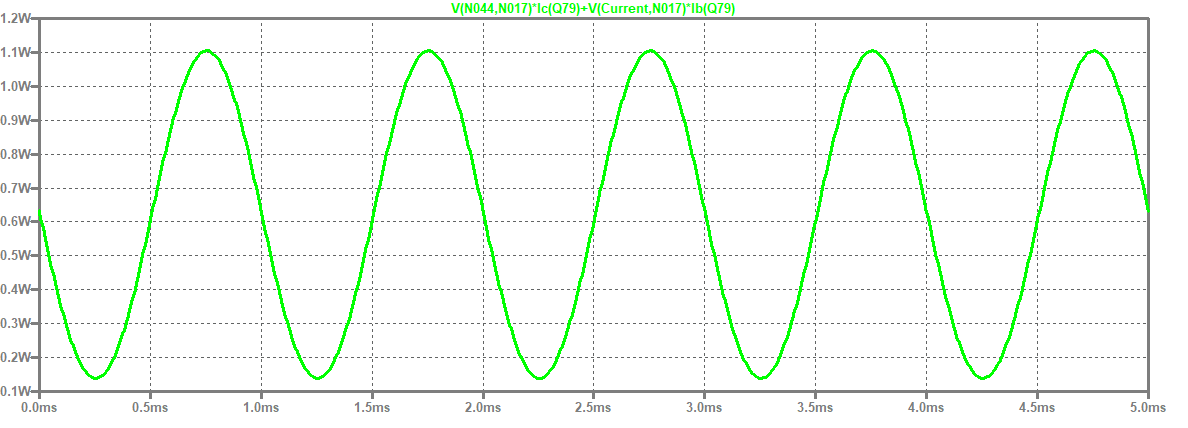
\includegraphics[width=0.8\textwidth]{ImagenesSimulaciones/PCSEC.png}
		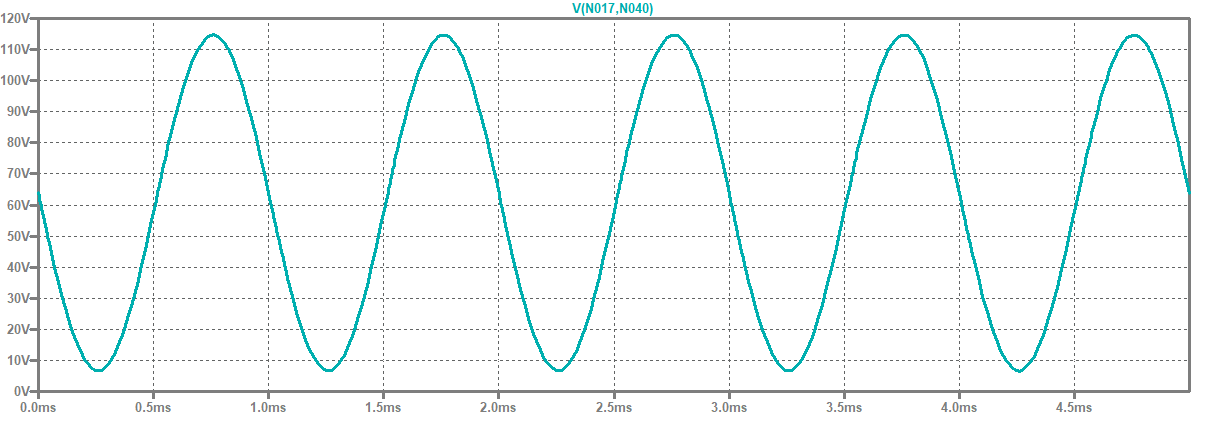
\includegraphics[width=0.8\textwidth]{ImagenesSimulaciones/VCSEC.png}
	\caption{Potencia y tensión sobre la carga activa.}
	\label{fig:pcsecf}
\end{figure}

%% potencia de la fuente de corriente del multiplicador de vbe
Continuando por la potencia y tensión correspondiente a la fuente de corriente de la etapa de salida.
\begin{figure}[H]
	\centering
	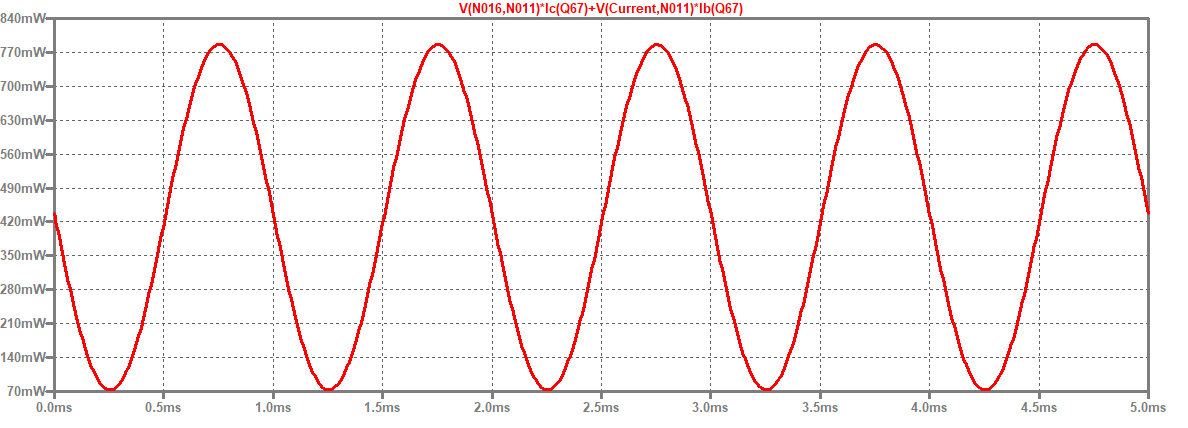
\includegraphics[width=0.8\textwidth]{ImagenesSimulaciones/PCSVBE.png}
		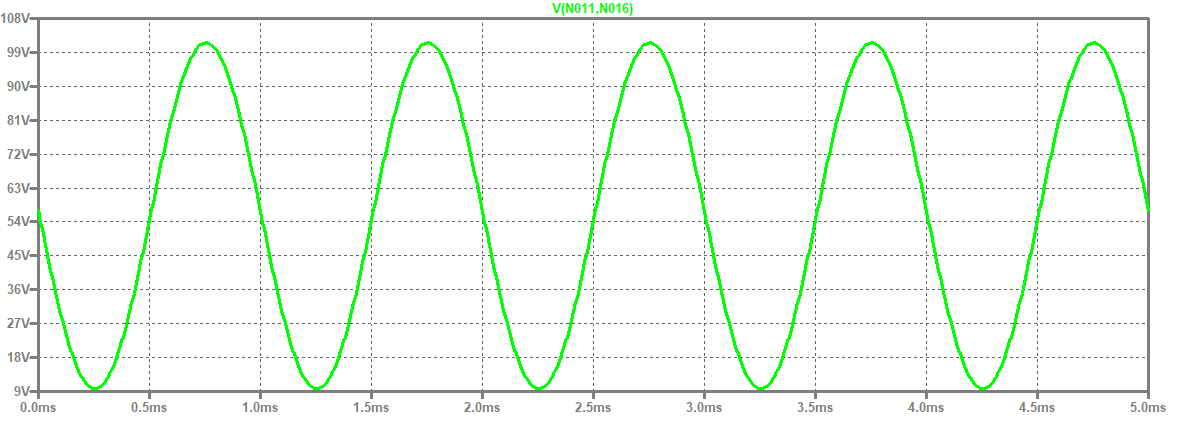
\includegraphics[width=0.8\textwidth]{ImagenesSimulaciones/VCSVBE.png}
	\caption{Potencia y tensión de la fuente de corriente de la salida.}
	\label{fig:pcsvbe}
\end{figure}
%%potencia en el primer transistor de salida
Considerando la potencia de la etapa de salida consideraremos la potencia de las 3 fases, correspondiendo a la primera, la de menor potencia:
\begin{figure}[H]
	\centering
	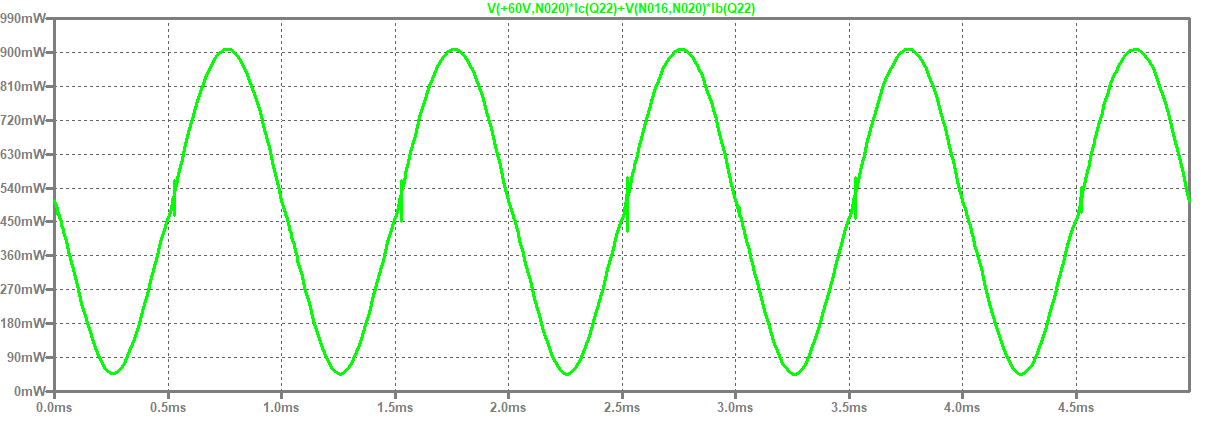
\includegraphics[width=0.8\textwidth]{ImagenesSimulaciones/PO1.png}
		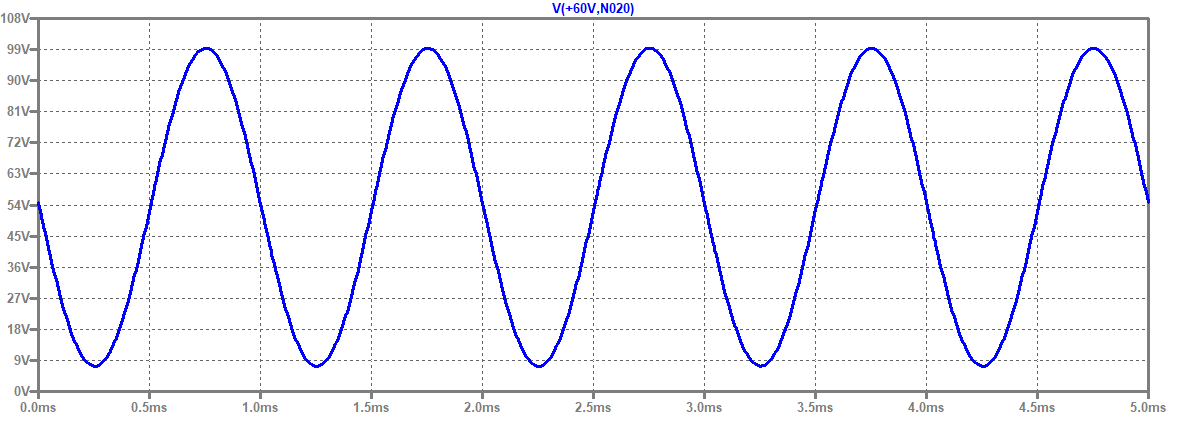
\includegraphics[width=0.8\textwidth]{ImagenesSimulaciones/VO1.png}
	\caption{Potencia y tensión del primer transistor de salida.}
	\label{fig:po1}
\end{figure}
Para el segundo, el cual corresponde a mediana potencia:
\begin{figure}[H]
	\centering
	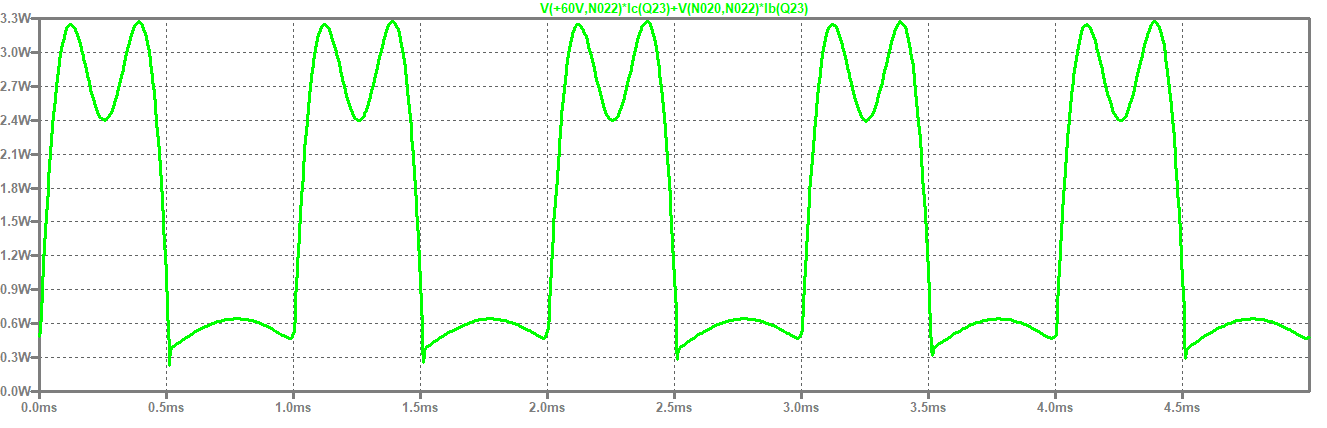
\includegraphics[width=0.8\textwidth]{ImagenesSimulaciones/PO2.png}
		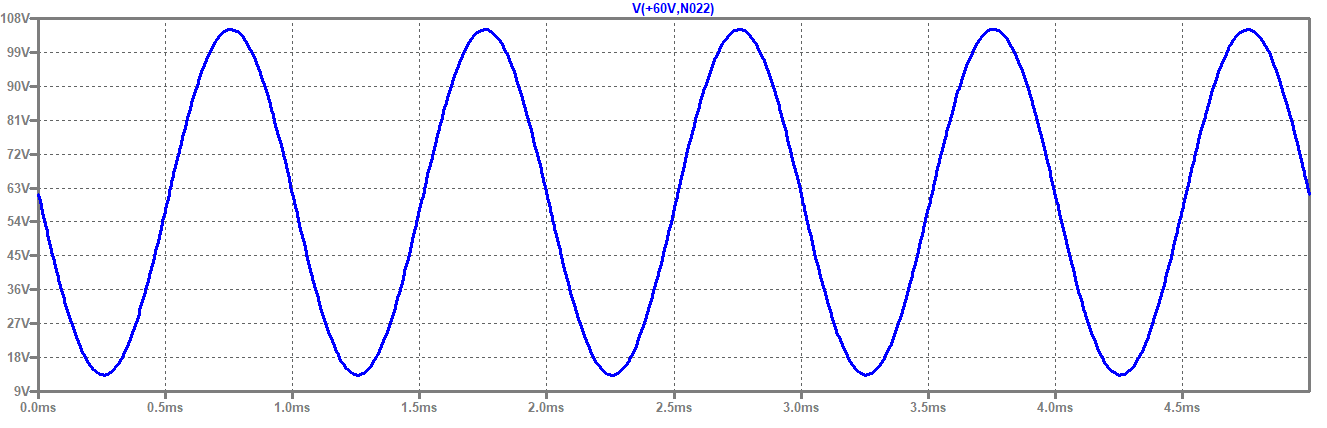
\includegraphics[width=0.8\textwidth]{ImagenesSimulaciones/VO2.png}
	\caption{Potencia y tensión del segundo transistor de salida.}
	\label{fig:po2}
\end{figure}
Finalmente para los últimos transistores, los cuales son los que trabajan con la mayor parte de la potencia de salida se obtuvo tanto la potencia como la tensión sobre ellos.
\begin{figure}[H]
	\centering
	\includegraphics[width=0.8\textwidth]{ImagenesSimulaciones/PO3.png}
		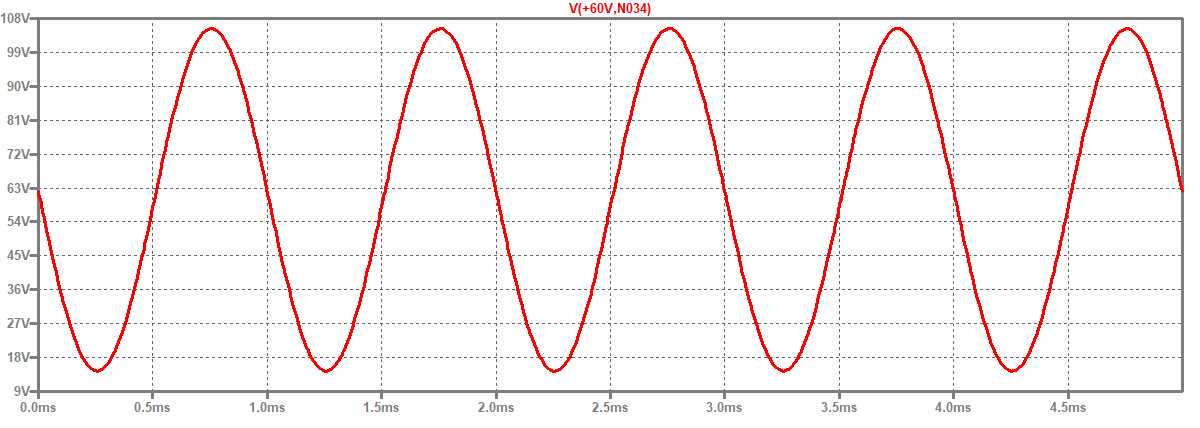
\includegraphics[width=0.8\textwidth]{ImagenesSimulaciones/VO3.png}
	\caption{Potencia y tensión de los transistores de salida.}
	\label{fig:po3}
\end{figure}
Adicional mente se puede observar que en el gráfico de potencias se dibujo también la potencia del transistor PNP de la rama inferior, para hacer evidente el nivel de simetría que se tiene.\\
Finalmente mostraremos la simulación de potencia sobre la carga.
\begin{figure}[H]
	\centering
	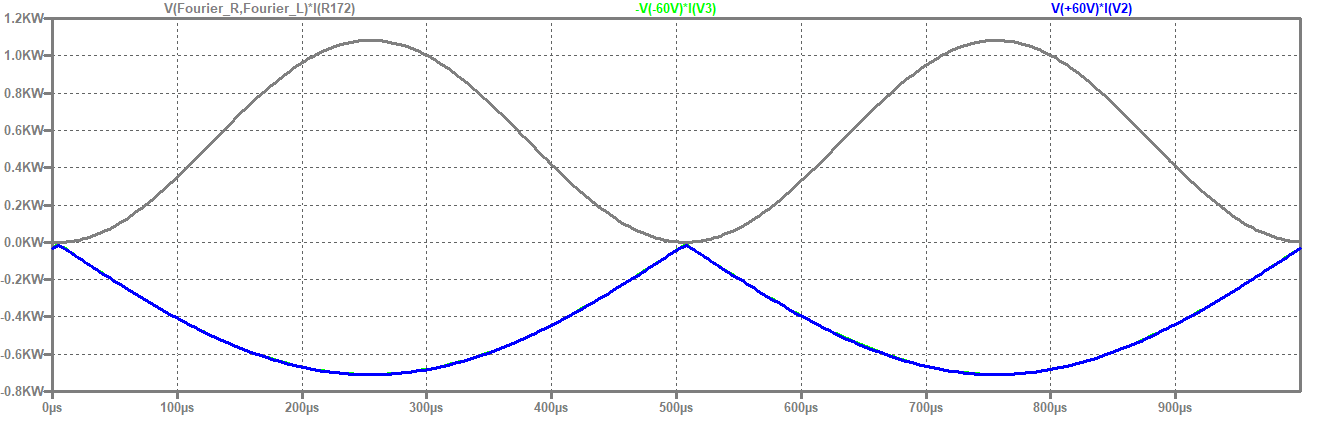
\includegraphics[width=0.8\textwidth]{ImagenesSimulaciones/PRL.png}
	\caption{Potencia sobre la carga.}
	\label{fig:porl}
\end{figure}
Aquí se pueden apreciar varias cosas, primeramente que con una tensión de entrada de 0.5$\hat{V}$ se obtiene la mayor potencia, la cual corresponde a $\approx 1078W$, también debe notarse que la potencia entregada por la fuente es $\approx 0W$ cuando la potencia sobre la carga también lo es.\\
Luego se obtuvo la salida del circuito teniendo a la entrada una señal senoidal de frecuencia 1KHz y de amplitud 0.25$\hat{V}$ y otra simulación con la misma entrada pero sumado también ruido blanco con distribución uniforme de amplitud $25m\hat{V}$.
\begin{figure}[H]
	\centering
	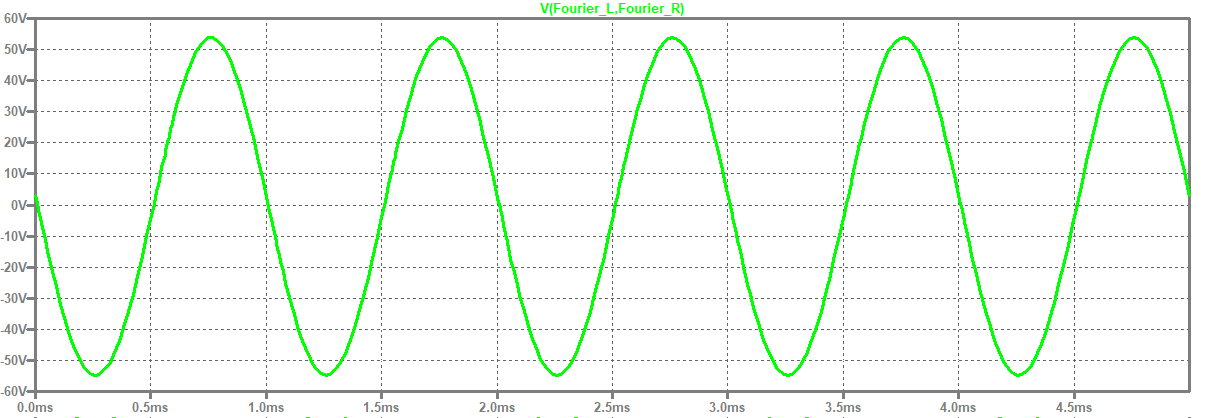
\includegraphics[width=0.8\textwidth]{ImagenesSimulaciones/VRL.png}
		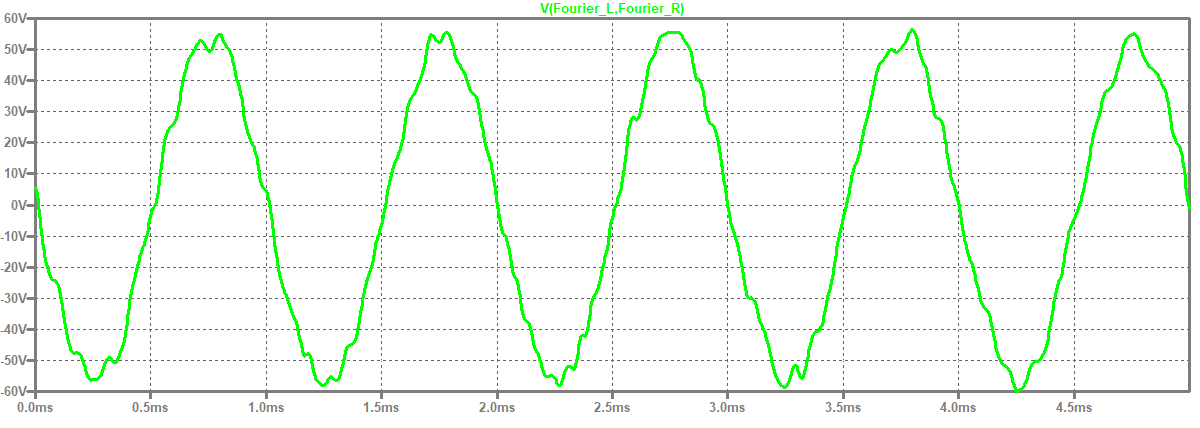
\includegraphics[width=0.8\textwidth]{ImagenesSimulaciones/VRLNoise.png}
	\caption{Tensión sobre la carga con y sin ruido.}
	\label{fig:VRLN}
\end{figure}
Finalmente se obtuvo el Bode del sistema como se observa a continuación:
\begin{figure}[H]
	\centering
	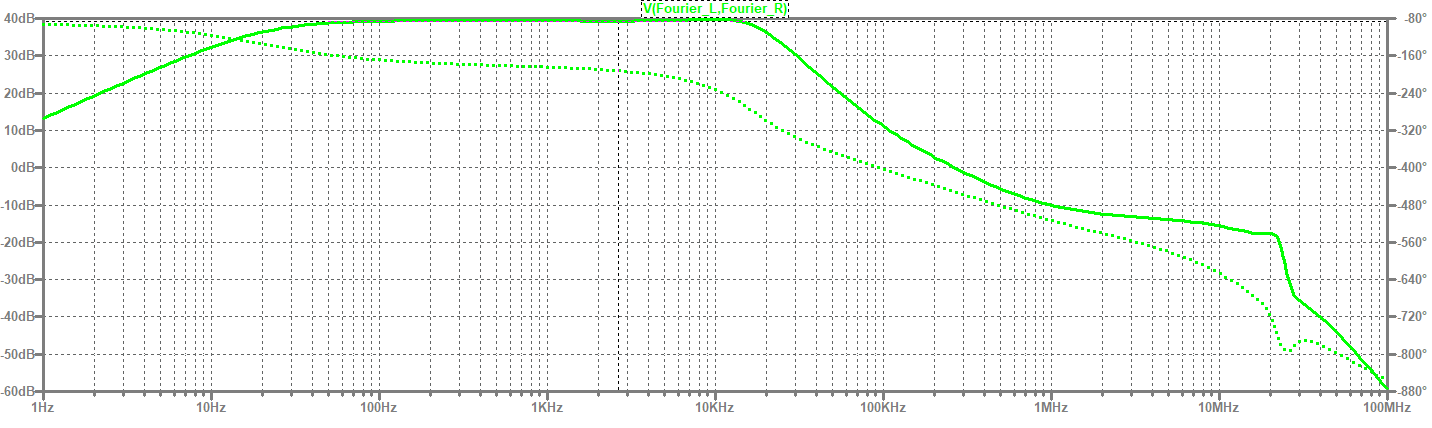
\includegraphics[width=0.9\textwidth]{ImagenesSimulaciones/BODE.png}
	\caption{Bode del sistema.}
	\label{fig:bode}
\end{figure}
Donde se puede apreciar una caida de 3dB respecto a la banda pasante tanto en 20Hz como en 20KHz.\\
También se simuló la impedancia tanto de entrada como de salida.
\begin{figure}[H]
	\centering
	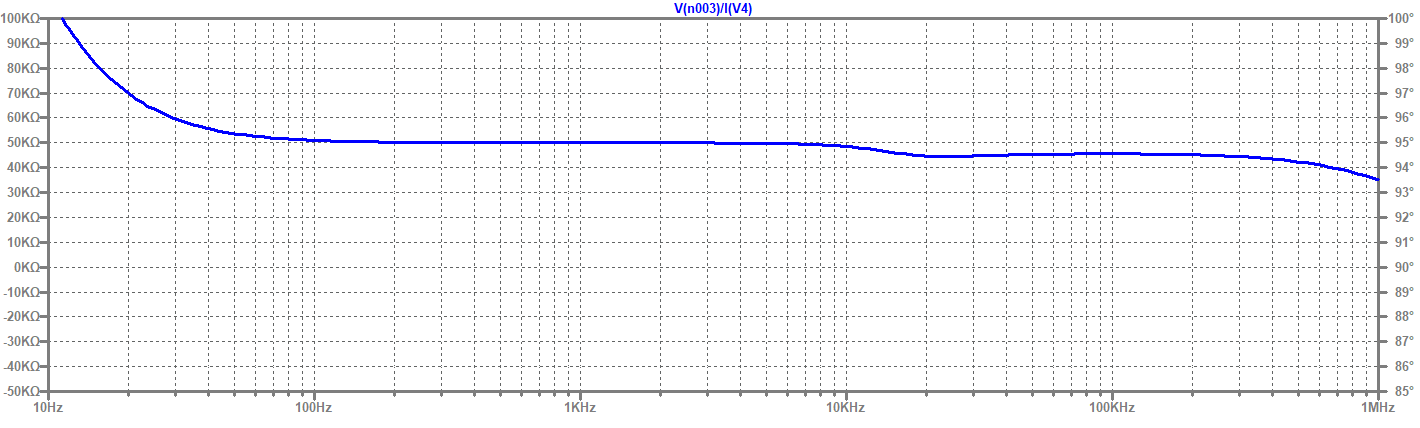
\includegraphics[width=0.9\textwidth]{ImagenesSimulaciones/Zin.png}
	\caption{Impedancia de entrada del sistema.}
	\label{fig:zin}
\end{figure}
Se puede notar que la impedancia de entrada en la banda audible es de 50K$\Omega$
\begin{figure}[H]
	\centering
	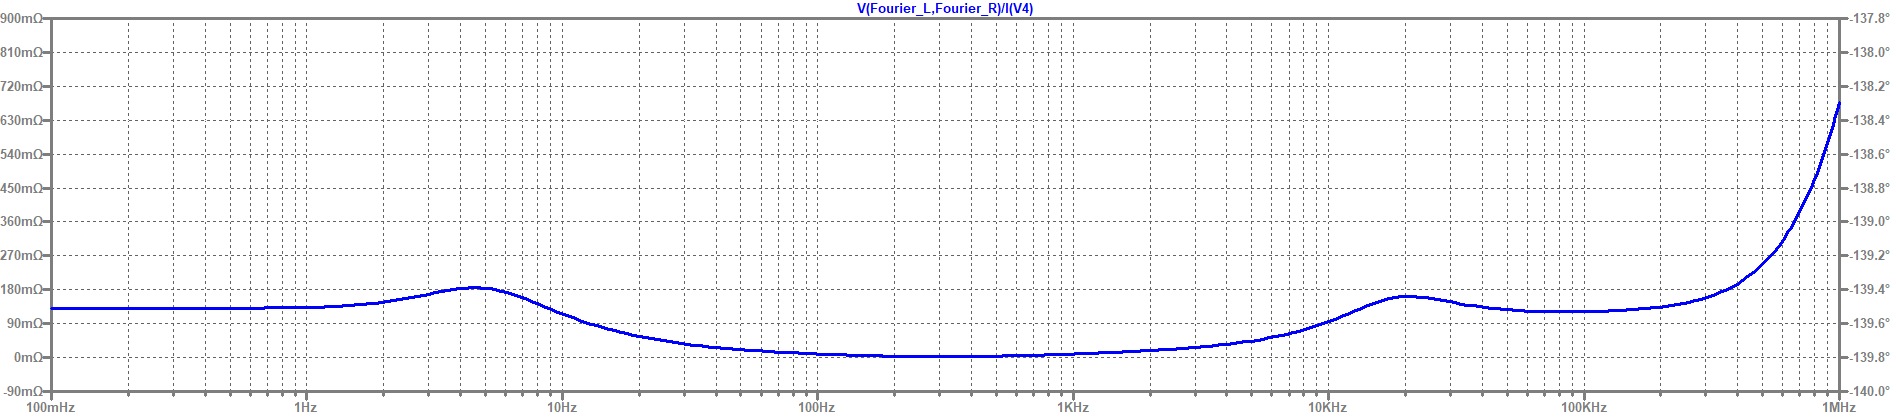
\includegraphics[width=0.9\textwidth]{ImagenesSimulaciones/Zout.png}
	\caption{Impedancia de salida del sistema.}
	\label{fig:zout}
\end{figure}
La impedancia de salida es un valor cercano del orden de las decenas de  m$\Omega$, idealmente sería de 8 $\Omega$ para que haya máxima transferencia de Potencia.
Como también se midió la THD en la simulación obteniendo un valor de 0.400742$\%$ cuando se disipa la máxima potencia.

\subsection{Efectos de la resistencia del Jfet}
Dado a que la resistencia del Jfet gobierna la corriente provista por el, variaciones en ella provocan un desvalance tanto en la tensión de salida, agregando un nivel de continua, como la potencia sobre los transistores de salida.\\
A continuación se muestra una simulación en la cual se puede apreciar el cambio de la tensión de salida provocado por la variación de dicha resistencia.
 \begin{figure}[H]
\centering
	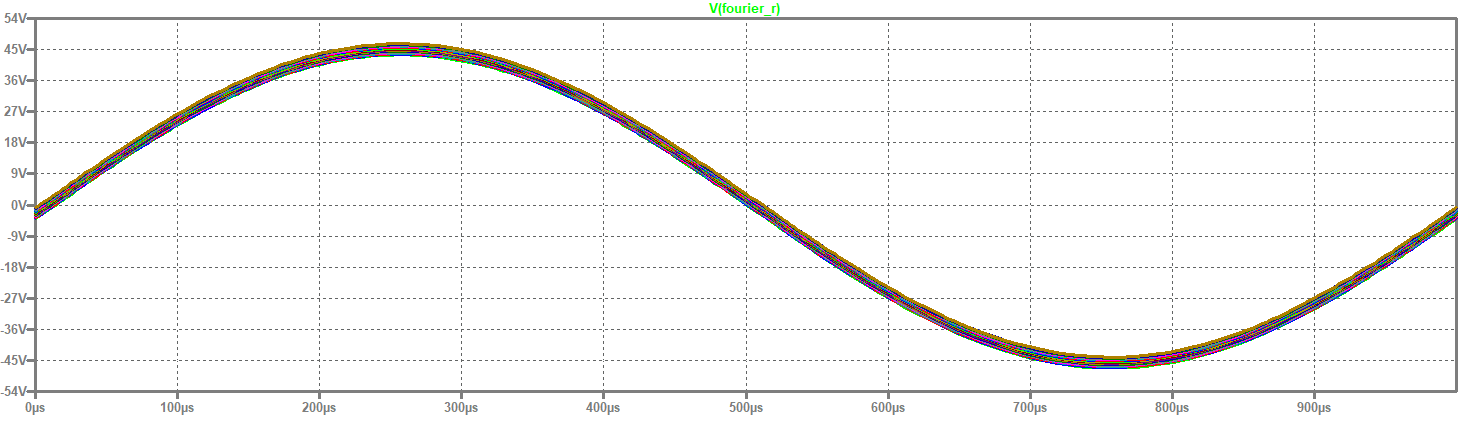
\includegraphics[width=0.7\textwidth]{ImagenesSimulaciones/jfetvar1.png}
	\caption{Variación de la tensión de salida en función de la resistencia del Jfet.}
	\label{fig:mcvl}
\end{figure}
El desvalance en la tensión de salida de cada etapa puede llegar a no ser un problema debido a la configuración de puente H. Teniendo la carga conectada diferencialmente, y al estar en contrafase ambas ramas del circuito, se cancelaría la continua sobre la carga, pero este nivel de continua que carga cada rama resulta un problema debido a que si la potencia disipada por los transistores esta desbalanceada, afecta seriamente al rendimiento.
 \begin{figure}[H]
\centering
	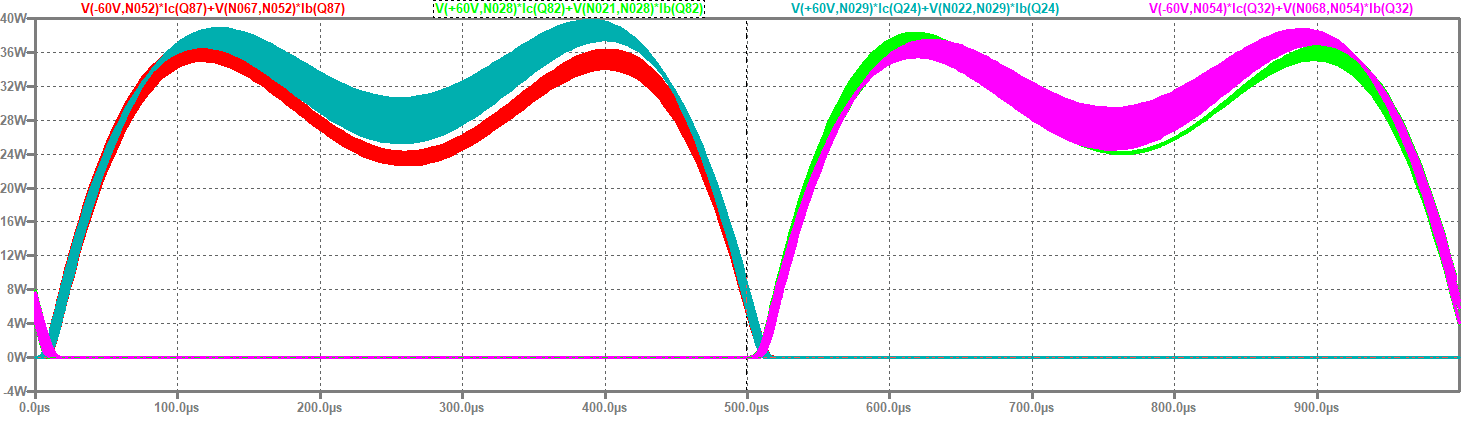
\includegraphics[width=0.7\textwidth]{ImagenesSimulaciones/DesvalanceP.png}
	\caption{Variación de la potencia de los transistores de salida en función de la resistencia del Jfet.}
	\label{fig:mcPl}
\end{figure} 

\section{Conclusiones}
	\label{simulaciones}
	%\documentclass[a4paper]{article}
\usepackage[utf8]{inputenc}
\usepackage[spanish, es-tabla, es-noshorthands]{babel}
\usepackage[table,xcdraw]{xcolor}
\usepackage[a4paper, footnotesep = 1cm, width=20cm, top=2.5cm, height=25cm, textwidth=18cm, textheight=25cm]{geometry}
%\geometry{showframe}

\usepackage{tikz}
\usepackage{amsmath}
\usepackage{amsfonts}
\usepackage{amssymb}
\usepackage{float}
\usepackage{graphicx}
\usepackage{caption}
\usepackage{subcaption}
\usepackage{multicol}
\usepackage{multirow}
\setlength{\doublerulesep}{\arrayrulewidth}
\usepackage{booktabs}

\usepackage{hyperref}
\hypersetup{
    colorlinks=true,
    linkcolor=blue,
    filecolor=magenta,      
    urlcolor=blue,
    citecolor=blue,    
}

\newcommand{\quotes}[1]{``#1''}
\usepackage{array}
\newcolumntype{C}[1]{>{\centering\let\newline\\\arraybackslash\hspace{0pt}}m{#1}}
\usepackage[american]{circuitikz}
\usetikzlibrary{calc}
\usepackage{fancyhdr}
\usepackage{units} 

\graphicspath{{../Calculos-Potencia/}{../Caracteristicas/}{../Consideraciones/}{../Gain-Stage/}{../Input-Stage/}{../Output-Stage/}{../Simulaciones/}{../Alimentacion/}{../Conclusiones/}}

\pagestyle{fancy}
\fancyhf{}
\lhead{22.12 Electrónica II}
\rhead{Mechoulam, Lambertucci, Rodriguez, Londero, Scala}
\rfoot{Página \thepage}

\begin{document}	

Se consiguió elaborar un amplificador para una carga nominal de $8 \ \Omega$, con una disipación máxima de $1.5 \ kW$ y una distorsión armónica no mayor a $0.529\%$. Es por ello que cabe preguntarse, ¿es posible mejorar el circuito?. Desde nuestro punto de vista, se llegó a la conclusión de que sí se puede mejorar ciertos parámetros, como por ejemplo, la distorsión armónica. La mejora propuesta consiste en el uso de amplificadores operacionales dentro del circuito. Estos permiten reducir el TDH a $0.015 \%$. Otra ventaja que presenta esta implementación es que se puede aplicar una realimentación negativa diferencial mediante el uso de la configuración sumador-restador. Este tipo de realimentación permite subir ..
	
\end{document}
	
\end{document}